\begin{filecontents*}{\jobname.xmpdata}
  \Title{Building a Ray-Traced Rendering Engine on Sparse Voxel Grids}
  \Author{10834225}
  \Language{en-GB}
  \Copyrighted{True}
\end{filecontents*}

\documentclass{extra}

%%%%%%%%%%%%%%%%%% PACKAGES AND COMMANDS %%%%%%%%%%%%%%%%%%
\usepackage{graphicx,psfrag,color} % for postscript graphics files
  \graphicspath{ {./figures/} }
\usepackage{amsmath}               % assumes amsmath package installed
  \allowdisplaybreaks[1]           % allow eqnarrays to break across pages
\usepackage{amssymb}               % assumes amsmath package installed
\usepackage{url}                   % format hyperlinks correctly
\usepackage{rotating}              % allow portrait figures and tables
\usepackage{multirow}              % allows merging of rows in tables
\usepackage{lscape}                % allows pages to be typeset in landscape mode
\usepackage{tabularx}              % allows fixed width tables
\usepackage{verbatim}              % enhanced version of built-in verbatim environment
\usepackage{footnote}              % allows more control over footnote environments
\usepackage{float}                 % allows H option on floats to force here placement
\usepackage{booktabs}              % improve table line spacing
\usepackage{lipsum}                % for adding dummy text here
\usepackage[base]{babel}           % for proper hypthenation in lipsum sections
\usepackage{subcaption}            % for multiple sub-figures in a single float
\usepackage{cleveref}
\usepackage{xcolor}
\usepackage{color}
\usepackage[inkscapelatex=false]{svg}
\usepackage[acronym]{glossaries}
\usepackage{listings}
\usepackage{listings-rust}
\usepackage{multicol}
\usepackage{bm}
\usepackage{enumitem}
\newtheorem{theorem}{Theorem}
\newcommand{\degree}{\ensuremath{^\circ}}
\newcommand{\sus}[1]{$^{\mbox{\scriptsize #1}}$} % superscript in text (e.g. 1st)
\newcommand{\sub}[1]{$_{\mbox{\scriptsize #1}}$} % subscript in text
\AtBeginEnvironment{quote}{\par\singlespacing\small}

%%%%%%%%%%%%%%%%%% REFERENCES SETUP %%%%%%%%%%%%%%%%%%
\usepackage[style=ieee,backend=biber,backref=true,hyperref=auto,backend=bibtex]{biblatex}
% \DefineBibliographyStrings{english}{backrefpage = {cited on p\adddot},  backrefpages = {cited on pp\adddot}}
\addbibresource{ref.bib}

\makeglossary
\newacronym{gcd}{GCD}{Greatest Common Divisor}

%%%%%%%%%%%%%%%%%% START DOCUMENT %%%%%%%%%%%%%%%%%%
\begin{document}
\makeatletter
\title{\xmp@Title}
\studentid{\xmp@Author}
\makeatother

\course{Computer Science}
\submitdate{2024}
\wordcount{many}
\maketitle



%%%%%%%%%%%%%%%%%% LISTS OF CONTENT %%%%%%%%%%%%%%%%%%
\uomtoc
% other lists are not required, but can include \uomlof and \uomlot if really want to


%%%%%%%%%%%%%%%%%% ABSTRACT %%%%%%%%%%%%%%%%%%
\begin{abstract} % put abstract here. Limit is 1 page.
  This is abstract text.

  \lipsum[1-2]
\end{abstract}%
\clearpage


%%%%%%%%%%%%%%%%%% DECLARATIONS %%%%%%%%%%%%%%%%%%
\uomdeclarations % Don't need unless final thesis


\begin{uomacknowledgements}
  Thanks!
\end{uomacknowledgements}

%%%%%%%%%%%%%%%%%% CONTENT %%%%%%%%%%%%%%%%%%
%%% Local Variables:
%%% mode: latex
%%% TeX-master: "../main"
%%% End:

\part{Introduction}
\section{Motivation}
\section{Aims}
\section{Objectives}
\section{Report structure}

%%% Local Variables:
%%% mode: latex
%%% TeX-master: "../main"
%%% End:

\part{Background and Literature Review}\label{backgorund}
\section{Rendering engines}
Graphics engines are the core software components responsible for rendering visual content in applications ranging from video games to scientific simulations and movie visual effects.
Engines abstract the complexities of rendering by providing developers with high-level tools and interfaces to represent digital environments.

Rendering engines have evolved from the simple wire-frame models of the 1960s to today's complex 3D systems, driven by advancements in computational power and graphical standards\cite{old} like OpenGL introduced in the early 1990s.

\subsection{Primitves}
At the heart of any graphical engine is the concept of primitives, the simplest forms of graphical objects that the engine can process and render. Primitives are building blocks from which more complex shapes and scenes can be constructed.

\textbf{Polygons}, particularly triangles, are the most commonly used primitives in 3D graphics. This is owed to their simplicity and flexibility, allowing the construction of virtually any 3D shape through \emph{tesselation}. Polygonal meshes define the surfaces of objects in a scene, with each polygon vertex typically associated with additional information such as colour, texture coordinates, and normal vectors for lighting calculations.

\textbf{Voxels} represent a different approach to defining 3D shapes; they are essentially three-dimensional pixels. Where polygons define surfaces, voxels establish volume, with each voxel potentially containing colour and density information.
This characteristic makes voxels particularly well-suited for rendering scenes with materials that have intricate internal structures, such as fog, smoke, fire, and fluids.

\subsection{Ray-tracing vs. Rasterization}
Rendering engines can utilise two main rendering techniques for rendering scenes: ray tracing and rasterisation. Both have advantages and trade-offs.

\textbf{Rasterization} is the most widespread technique used in real-time applications.
It converts the 3D scene into a 2D image by projecting vertices onto the screen, filling in pixels that makeup polygons, and applying textures and lighting.
Over the development of the graphics programming industry, graphics hardware has become extremely efficient at performing rasterisation, making it the standard for video games and interactive applications.

\textbf{Ray-Tracing}, in contrast, simulates the path of light as rays travelling through a scene to produce images with realistic lighting, shadows, reflections, and refractions. Ray tracing is computationally intensive but yields higher-quality images, making it favoured for applications where visual fidelity is critical. However, recent advancements in hardware have begun to bring real-time ray tracing to interactive applications.

Ray tracing, conceptualised by Arthur Appel in 1968\supercite{appel}, offers photorealistic images by simulating light paths, but its computational intensity limited early use to non-real-time applications. Rasterisation, popularised in the 1970s and optimised by GPU advancements, became the standard for real-time graphics, though \emph{recent} hardware innovations are now enabling real-time ray tracing.

\section{Representing voxels}
Various data structures can be employed to represent and manipulate voxels in program memory efficiently. Each method entails trade-offs between memory usage, access speed, and implementation complexity. Access speed refers to the time complexity of querying the data structure at an arbitrary point in space to retrieve a potential voxel.

\subsection{Voxel grids}
A voxel grid is the most straightforward and intuitive approach to representing volumetric data. The 3D space is divided into a regular grid of voxels, each holding information such as colour, material properties, or density. This method provides direct $O(1)$ access to voxel data.

However, this simplicity comes at a significant disadvantage: memory consumption.
As the bounding volume or the level of detail of the scene increases, the memory required to store the voxel grows by $O(N^{3})$.
Additionally, empty space can occupy a majority of the memory space.
For example, consider a scene with two voxels a million units apart in all axes.
A voxel grid would have to store all the empty voxels in-between; $10^{18}$ memory units reserved, 2 of which carry useful data.
This limitation makes the naive voxel grids impractical for large or highly detailed scenes.

\subsection{Hierarchical voxel grids (N-trees)}
Hierarchical grids, such as octrees, are employed to mitigate these issues. An octree is a tree data structure where each node represents a cubic portion of 3D space and has up to eight children. This division continues recursively, allowing for varying levels of detail within the scene: larger volumes are represented by higher-level nodes, while finer details are captured in lower levels.

The primary advantage of using an octree is spatial efficiency. Regions of the space that are empty or contain uniform data can be represented by a single node, significantly reducing the memory footprint. Furthermore, octrees facilitate efficient querying operations, such as collision detection and ray tracing, by allowing the algorithm to discard large empty or irrelevant regions of space quickly.

Hierarchical grids introduce complexity in terms of implementation and management. Operations such as updating the structure or balancing the tree to ensure efficient access can be more challenging than those of uniform grids.
Another sacrifice is access time, as querying an arbitrary region of space can entail walking down the tree for several levels.
Nonetheless, the benefits of hierarchical representations often outweigh these drawbacks for applications requiring large, detailed scenes with a mix of dense and sparse regions. Therefore, N-trees are frequently used in voxel engines.

Donald Meagher introduced the concept of octrees in 1980\supercite{donald} as a means to manage spatial data in 3D computer graphics efficiently. This technique quickly became integral in applications like 3D rendering and geometric modelling, where it revolutionized spatial data optimization by balancing detailed representation with computational efficiency.

\subsection{VDB}
\newacronym{bpt}{B+tree}{A m-ary tree with a variable but often large number of children per node.}
\newacronym{vdb}{VDB}{Volumetric Dynamic B+tree grid data structure introduced by Ken Museth\supercite{vdb2013}}

\textbf{\acrshort{vdb}} was introduced in 2013 by Ken Museth\supercite{vdb2013} from the DreamWorks Animation team.
\begin{quote}
It is a Volumetric, Dynamic grid that shares several characteristics with B+trees.
It exploits spatial coherency of time-varying data to separately and compactly encode data values and grid topology.
VDB models a virtually infinite 3D index space that allows for cache-coherent and fast data access into sparse volumes of high resolution.
\end{quote}

At its core, VDB functions as a shallow N-tree with a fixed depth, where nodes at different levels vary in size. The top level of this tree structure is managed through a hash map, enabling VDB models to cover extensive index spaces with minimal memory overhead. This design achieves $O(1)$ access performance and effectively stores tiled data across vast spatial regions.

The VDB data structure was introduced along with several algorithms that fully use the data structure's features, offering significant improvements in techniques for efficiently rendering volumetric data. These are some of VDB's benefits, as detailed in the original paper.
\begin{enumerate}
  \item \emph{Dynamic}. Unlike most sparse volumetric data structures, VDB is developed for both dynamic topology and dynamic values typical of time-dependent numerical simulations and animated volumes.
  \item \emph{Memory effcient}. The dynamic and hierarchical allocation of compact nodes leads to a memory-efficient sparse data structure that allows for extreme grid resolution.
  \item \emph{Fast random and sequential data access}. VDB supports fast, constant-time random data lookup, insertion, and deletion.
  \item \emph{Virtually infinite}. VDB, in concept, models an unbounded grid in the sense that the accessible coordinate space is only limited by the bit-precision of the signed coordinates.
  \item \emph{Efficient hierarchical algorithms.} The \acrshort{bpt} structure offers the benefits of cache coherency, inherent bounding-volume acceleration, and fast per-branch (versus per-voxel) operations.
\end{enumerate}
These benefits make VDB a very compelling data structure that serves as the building block of a voxel-based rendering engine.

\section{Ray tracing}
To render a scene using ray tracing, camera rays are shot through the view frustum and into the scene. At each object intersection, part of a ray is absorbed, reflected, and refracted. To achieve realistic results, a rendering engine needs to model as many of these light interactions as possible in each frame's time budget.

This section delves into integrating ray tracing within the graphics pipeline and the methods used to implement it, focusing on casting a ray through a scene.

\subsection{Graphics pipeline}
The graphics pipeline of a rendering engine is the underlying system of a rendering engine that transforms a 3D scene into a 2D representation that is then presented on a screen. While rasterization transforms 3D objects into 2D images through a series of stages(vertex processing, shape assembly, geometry shading, rasterization, and fragment processing), the ray tracing pipelines introduce a paradigm shift. It primarily involves calculating the path of rays from the eye (camera) through pixels in an image plane and into the scene, potentially bouncing off surfaces or passing through transparent materials before contributing to the colour of a pixel.

Calculating a ray's path is central to ray tracing, so the performance of the algorithm that does this calculation is critical.
\subsection{Casting a ray}
Ray casting techniques vary depending on the representation of the 3D world within the rendering engine.
This section introduces basic ray casting techniques, while subsequent discussions cover methods specific to voxel-based environments.

\vspace{0.5cm}
\textbf{Ray marching}

A straightforward way to represent a 3D environment would be a mathematical function of sorts.
It would take the coordinates of a point as input and return the material's properties at that point (provided an object is present).

The first algorithm one might develop when trying to cast a ray through an unknown scene is ray marching.
It involves incrementally stepping along a ray, sampling the scene for collisions at each step.
The chosen step size must be sufficiently small to ensure no detail is missed.

While simple, ray marching has drawbacks, especially in terms of performance.
Considering the need to process millions of pixels per frame within the time constraints of high frame rates, it becomes apparent that iterating a ray tens of thousands of times for every pixel is impractical for modern engines.

These constraints require exploring more advanced techniques to meet the goal of visual realism and performance.

\vspace{0.5cm}
\textbf{Ray casting}

A 3D environment could also be represented as a collection of polygons that form meshes.

Ray casting finds the intersection of rays with geometric primitives (e.g. triangles and circles). This method skips stepping along the ray entirely by using the underlying mathematics of intersecting lines with polygons.

The fundamental issue with this approach is that rays must be checked for an intersection with all the primitives in the scene. Thus, computing a single ray's intersection has linear complexity in terms of the number of polygons in the scene.


\vspace{0.5cm}
\phantomsection\label{def:sdf}
\textbf{SDF}
\newacronym{sdf}{SDF}{Signed distance fields, described in \cref{def:sdf}}

Signed distance fields (\acrshort{sdf}) are a different way of representing the environment. An SDF provides the minimum distance from a point in space to the closest surface, allowing the ray marching algorithm to skip empty space and efficiently determine surface intersections.
With the distance to the nearest surface known, ray marching can be performed by stepping along the ray with that distance, drastically reducing the number of steps needed to cast a ray.

Combining SDF with ray marching offers a powerful method for rendering complex scenes, including soft shadows, ambient occlusion, and volumetric effects.
This combination is highly flexible and can create highly detailed and intricate visual effects, particularly in procedural rendering and visual effects.

SDFs are not without drawbacks. They can be difficult to maintain and computationally expensive to generate or update. In practice, distance data cannot be of arbitrary size, as that distance information comes at the cost of program memory.

SDFs have been used in real-time rendering, usually in a raymarching context, starting in the mid-2000s. In 2007, Valve used SDFs to render large pixel-size smooth fonts on the GPU in its games\supercite{valve}.

\subsection{Casting a ray on a voxel grid}
The ray casting methods presented so far do not take advantage of the discrete voxel grid on which this rendering engine is based. This section presents efficient algorithms that can use the underlying representation of a hierarchical voxel grid.

\vspace{0.5cm}
\phantomsection\label{def:dda}
\textbf{DDA}
\newacronym{dda}{DDA}{Digital Differential Analyzer, line drawing algorithm described in \cref{def:dda}}

Basic ray marching can be improved on a discrete voxel grid by stepping from voxel to voxel. Because voxels are the smallest unit of space, a ray can safely step from one to the next, ensuring there is nothing else in between.

The Digital Differential Analyzer (\acrshort{dda}) line drawing algorithm does precisely that; it marches along a ray from voxel to voxel, skipping all space in between.

DDA works by breaking down the minimum distance a ray travels to intersect a grid line on each axis.
At each iteration, it steps to the closest grid intersection along the ray.

\vspace{0.5cm}
\phantomsection\label{def:hdda}
\newacronym{hdda}{HDDA}{Hierarchical \acrshort{dda}, line drawing algorithm described in \cref{def:hdda}}
\textbf{HDDA}

On a hierarchical grid, the DDA algorithm can take advantage of the data structure's topology by stepping through empty, larger chunks.
A ray cast using \acrshort{hdda} essentially performs DDA at the level in the tree it is currently at.

Ken Museth introduced a version of the HDDA algorithm for the VDB data structure in 2014\supercite{vdb2014}.
This algorithm can be highly efficient; large empty areas can be skipped in a single step, drastically reducing the required steps to march a ray.

\section{Summary of similar systems}
\subsection{OpenVDB\supercite{openvdb:doc}}

\begin{quote}
``OpenVDB is an Academy Award-winning open-source C++ library comprising a novel hierarchical data structure and a suite of tools for the efficient storage and manipulation of sparse volumetric data discretized on three-dimensional grids. It was developed by DreamWorks Animation for use in volumetric applications typically encountered in feature film production and is now maintained by the Academy Software Foundation (ASWF).
''
\end{quote}

This voxel rendering engine is made on the same backend as this project, Rust and wgpu. However, it employs a more standard approach to rendering, generating triangle meshes from voxel data and performing rasterization.

\subsection{All is Cubes\supercite{cubes}}

\begin{quote}
``This project is a game engine for worlds made of cubical blocks (“blocky voxels”). The particular features of this engine are that each ordinary block is itself made out of blocks, and all game mechanics are defined by data within the world that can be interactively edited.''
\end{quote}

This is a voxel rendering engine made on the same backend as this project, Rust and wgpu, however it employs a more standard apprach of rendering, generating triangle meshes from voxel data and performing rasterization.

\subsection{ Unique Contribution of this Project}
To the best of my knowledge, there is currently no fully operational voxel rendering engine built solely on the VDB data structure. This project aims to fill that gap by developing a comprehensive rendering engine based entirely on VDB, leveraging its capabilities to efficiently handle complex and detailed volumetric data. Unlike other systems, which may integrate VDB as one of many components or use it for specific functions, this engine is designed to utilize VDB as the core framework for all rendering tasks. This distinction sets the project apart, offering a new perspective and opportunities to explore novel ray-tracing techniques.

%%% Local Variables:
%%% mode: latex
%%% TeX-master: "../main"
%%% End:

\section{Methodology}
This section outlines the implementation details of the voxel rendering engine, starting from the selection of programming languages and libraries, going over the architecture of the engine, and diving deep into the data structures and algorithms employed, particularly focusing on VDB for voxel representation and the optimization of ray casting algorithms.
Finally, this section will discuss the extension of these algorithms to full-fledged ray tracing, allowing for dynamic lightning and glossy material support.

\subsection{Rust \& Wgpu}
\hyphenation{WebGPU}

The voxel rendering engine is built using \textbf{Rust}, a programming language known for its focus on safety, speed, and concurrency\supercite{rustbook}.
Rust's design emphasizes memory safety without sacrificing performance, making it an excellent choice for high-performance applications like a rendering engine.
The language's powerful type system and ownership model prevent a wide class of bugs, making it ideal for managing the complex data structures and concurrency challenges inherent in rendering engines. Thanks to this no memory leak or null pointer was ever encoutered throughout the developmenent of this project.

For the graphical backend, the engine utilizes \textbf{wgpu}\supercite{wgpu}, a Rust library that serves as a safe and portable graphics API. wgpu is designed to run on top of various backends, including Vulkan, Metal, DirectX 12, and WebGL, ensuring cross-platform compatibility. This API provides a modern, low-level interface for GPU programming, allowing for fine-grained control over graphics and compute operations. wgpu is aligned with the WebGPU specification\supercite{webgpu:doc}, aiming for broad support across both native and web platforms.
This choice ensures that the engine can leverage the latest advancements in graphics technology while maintaining portability and performance.

The combination of Rust and wgpu offers several advantages for the development of a rendering engine:

\begin{enumerate}
  \item \emph{Safety and Performance:} Rust’s focus on safety, coupled with wgpu's design, minimizes the risk of memory leaks and undefined behaviors, common issues in high-performance graphics programming. This is thanks to Rust's idea of zero-cost abstractions.

  \item \emph{Cross-Platform Compatibility:} With wgpu, the engine is not tied to a specific platform or graphics API, enhancing its usability across different operating systems and devices.

  \item \emph{Future-Proofing:} wgpu's adherence to the WebGPU specification ensures that the engine is built on a forward-looking graphics API, designed to be efficient, powerful, and broadly supported. It also allows the future option of supporting web platforms, once browsers adopt WebGPU more throughly.

  \item \emph{Concurrency:} Rust’s advanced concurrency features enable the engine to efficiently utilize multi-core processors, crucial for the heavy computational demands of rendering pipelines.
\end{enumerate}

These technical choices form the foundation upon which the voxel rendering engine is constructed. Following this, the engine's architecture is designed to take full advantage of Rust's performance and safety features and wgpu's flexible, low-level graphics capabilities, setting the stage for the implementation of advanced voxel representation techniques and optimized ray tracing algorithms.


\subsection{Engine architecture}
\subsubsection{Runtime}
\newacronym{os}{OS}{Operating System}
\begin{samepage}
At the engine's core, sits \texttt{Runtime}  structure, which manages the interaction between the it's main components:
\begin{itemize}
  \item The \texttt{Window} is a handler to the engine's graphical window. It is used in filtering \acrshort{os} events that relevant to engine, grabbing the cursor and other boilerplate.
  \item The \texttt{Wgpu Context} holds the creation and application of the rendering pipeline.
  \item The \texttt{Scene} contains information abput the camera and enviorment as well as a container voxel data structure.
\end{itemize}
\end{samepage}

\begin{lstlisting}[language=rust,caption={Runtime definition},captionpos=b]
pub struct Runtime {
  context: WgpuContext,
  window: Window,
  scene: Scene,
}

impl Runtime {
  ...
  pub fn main_loop(&mut self, event: Event, ...) {
    match event {
      ...
    }
  };
}
\end{lstlisting}

The engine's operation is centered around an event-driven main loop that blocks the main thread.
This loop processes various events, ranging from keyboard inputs to redraw requests, and updates the window, context, and scene accordingly, roting each event to it's corresponding handler.

For example, window events (e.g. keyboard \& mouse input) generaly modify the scene, like the camera position, and therfore are routed to the \verb|Scene| struct.

Another key event is the \verb|RedrawRequested| event, which signals that a new frame should be rendered. This is routed to the wgpu context to start the rendering pipeline.

\subsubsection{WgpuContext}
The WgpuContext structure forms the backbone of the rendering pipeline in the voxel rendering engine. It encapsulates the necessary components for interfacing with the GPU using the wgpu API, managing resources such as textures, shaders, and buffers, and executing rendering commands. This structure facilitates the integration of complex rendering techniques, including the handling of volumetric data through VDB and optimized ray casting for voxel environments.

The main components and functionalities of WgpuContext include:

Graphics API Integration: Initializes and configures the wgpu::Device and wgpu::Queue, along with a wgpu::Surface for rendering output. These components are crucial for executing GPU operations and presenting the rendered images.
Resource Management: Manages various GPU resources such as Texture, Buffer, and ShaderModule objects. This includes the setup of texture atlases for voxel data, uniform buffers for shader inputs, and dynamic shader loading and compilation.
Rendering Pipeline Configuration: Constructs the rendering pipeline with customized BindGroup and Pipeline configurations tailored to voxel rendering. This setup enables efficient processing and rendering of volumetric data.
Event-Driven Rendering Control: Implements methods to handle resizing events and rendering requests, adjusting the viewport and reconfiguring the pipeline as needed.
Volumetric Data Handling: Integrates with VDB to load, process, and render volumetric data, including the generation of signed distance fields (SDF) and the management of voxel atlases.
GUI Integration: Incorporates EguiDev for GUI rendering over the 3D scene, allowing for interactive model selection and parameter adjustments.
Asynchronous and Concurrent Execution: Utilizes tokio::runtime for asynchronous operations and concurrency management, facilitating non-blocking GPU resource operations and efficient data processing.
Key implementations derived from the source code:

Initialization and Configuration: The new async function initializes the WgpuContext by setting up the wgpu instance, device, queue, and surface. It also configures the surface with the desired format and dimensions, preparing the context for rendering.
Resource Setup: The constructor prepares various resources such as textures for the atlas representation of VDB data, uniform buffers for rendering state, and bind groups for shader inputs. It also dynamically reads VDB files, processes the data, and updates GPU resources accordingly.
Rendering Execution: The render method orchestrates the rendering process. It triggers compute shaders for voxel data processing, manages texture and buffer updates, and executes the render pipeline to draw the scene. Additionally, it integrates GUI rendering and handles screen capture for recording.
Shader Management: Provides mechanisms for loading and reloading shaders at runtime, allowing for dynamic updates to the rendering logic without restarting the application.
Event Handling and Interaction: Includes functions for responding to window and input events, adjusting the rendering context based on user actions such as resizing the window or changing the viewed model.
The WgpuContext architecture demonstrates a comprehensive approach to managing the complexities of rendering voxel-based scenes with ray tracing. It leverages modern GPU programming techniques, efficient data structures, and asynchronous processing to achieve high-performance rendering of volumetric data, while also providing a flexible platform for future enhancements and optimizations.



\subsubsection{Graphichs Pipeline}
\subsubsection{GPU Types}
\subsubsection{Camera}
\subsubsection{Shaders}
\subsubsection{Utilities}

\subsection{VDB Implementation}

%\subsection{VDB Implementation}

In this section the theory and implementation the VDB data structure is covered.

The VDB (Volumetric Dynamic B-tree) is an advanced data structure designed for efficient and flexible representation of sparse volumetric data. It is organized hierarchically, consisting of root nodes, internal nodes, and leaf nodes, each serving distinct purposes within the structure. This section begins by explaining in detail how VDB is structured, and it continues by going though the implementation of the data structure in the rendering engine.

\subsubsection{Data Structure}
VDBs are sparse, shallow trees with a fixed depth but expandable breadth, capable of covering an virutally infinite spatial domain. This design enables the VDB to efficiently manage large and complex datasets by adjusting the level of detail dynamically and minimizing memory usage.

\begin{figure}[H]
  \centering
  \includegraphics[width=\linewidth]{vdb}
  \caption{2D \& 1D slices of the VDB data structure representing three quarters of a circle. Top left: 2D dense representation of the circle. Top right: 2D sparse representation of the VDB. Bottom left: Sparse representation of the 1D vdb. Usually, VDB nodes have many more child nodes, which whould make it harder to visualise, hence a smaller version of VDB is shown. This figure is an augumented version of the one in the original paper\supercite{vdb2013}}
\end{figure}

At the hear of the data structure are its three types of nodes, internal root and leaf. The VDB data structure is inherently general, each of the nodes' sizes can be modefied depending on the application. However, in practice only one specialization of the VDB structure is used, that is the VDB345. This is because the authors of the original paper\supercite{vdb2013} analyized a suite of possible shapes and sizes, and this configuration of VDB the most balanced between performance and memory footprint for most practical applications [TODO: what applications?]

\paragraph{Leaf Nodes} They are the lowest level in the tree structure. They store a 3D cubed grid of side length $2^{\log_{2} D}$ (i.e. only powers of 2). An leaf value in the grid can be a voxel's data, other associated data for empty values (such as SDF information), or an empty value.
Leaf nodes also store a value mask. This is a bit-array meant to compactly determine if value at a specific coordinate in the 3D grid is voxel data or an empty value.

In the implementation the trait \verb|Node| is defined which gives some associated data and methods leaf and internal nodes have.

\begin{lstlisting}[language=rust,caption={\texttt{Node} trait definition},captionpos=b,label={code:node}]
pub trait Node {
    /// LOG2_D of side length
    /// LOG2_D = 3 => `512 = 8 * 8 * 8` values
    const LOG2_D: u64;
    /// Total conceptual LOG2_D node
    const TOTAL_LOG2_D: u64;
    /// Total conceptual LOG2_D of child node
    const CHILD_TOTAL_LOG2_D: u64 = Self::TOTAL_LOG2_D - Self::LOG2_D;
    /// Side length
    const DIM: u64 = 1 << Self::LOG2_D;
    /// Total conceptual dimension
    const TOTAL_DIM: u64 = 1 << Self::TOTAL_LOG2_D;
    /// Size of this node (i.e. length of data array)
    const SIZE: usize = 1 << (Self::LOG2_D * 3);
    /// Total conceptual size of node, including child size
    const TOTAL_SIZE: u64 = 1 << (Self::TOTAL_LOG2_D * 3);
}
\end{lstlisting}

In \cref{code:node}, \verb|TOTAL_LOG2_D| represents the $\log_{2}$ of the total dimension of the node, meaning how much actual space the node occupies. Leaf nodes are at the bottom of the tree and don't have children so this is the same as $\log_{2} D$, but this value will be relevant for internal nodes. All other attributes are determined at compile-time depending on the size of the node $\log_{2} D$.

\begin{quote}
  \paragraph{Sidenote on Coordinate Systems}

  It is very convenient for side lengths to be powers of two because of the way integers are stored in memory, as binary values. To get the global coordinate of a node with \verb|TOTAL_LOG2_D| $= 3$ that contains a point in global coordinates, the 3 least signifcant bits of each coordinate have to be masked out. This can essentially be done in a single CPU instruction for each coordinate.

\begin{lstlisting}[language=rust]
/// Give global origin of Node coordinates from `global` point
fn global_to_node(global: GlobalCoordinates) -> GlobalCoordinates {
    global.map(|c| (c >> Self::TOTAL_LOG2_D) << Self::TOTAL_LOG2_D)
}
\end{lstlisting}

Simillary, to get the relative coordinates of a global point within the node are precisely the \texttt{TOTAL\_LOG2\_D} least siginificant bits.

\begin{lstlisting}[language=rust]
/// Give local coordinates relative to the Node containing `global` position
fn global_to_relative(global: GlobalCoordinates) -> LocalCoordinates {
    global.map(|c| (c & ((1 << Self::TOTAL_LOG2_D) - 1)))
}
\end{lstlisting}

This pattern of a few bit-wise operations can acheive any conversion from between coordinate systems one might need, and all of these through operations are extremly fast to compute on modern CPUs.
\end{quote}

\Cref{code:leaf} shows a simplified definition of the leaf node data structure in the implementation. It has two fields: data which is an array representing the 3D cube grid of values, and value mask which is a the bit-mask carrying information on what each value represnts, a voxel or empty space. the data array has has $2^{3\log_{2} D}$ entries(e.g. for $\log_{2} D = 3 \Rightarrow D = 8$ the leaf node has $8\times8\times8 = 512 = 2^{9}$ values). The value mask has the same number of bit entries, but it is stored as an array of unsined 64 bit integers, hence there are $\frac{D^{3}}{64}$ of them.

\begin{lstlisting}[language=rust, captionpos=b, caption={
    \texttt{LeafNode} definition.
    In the original paper\supercite{vdb2013} node data is set as a union instead of a enum, in order to save on memory space, only using the masks to determine the type of a particular values.
    In this implementation a enum is used strictly for \emph{ergonomics}, as the extra 1 byte of memory per value is generally not expensive on heap allocated memory.
    The value mask will still be curcial for the GPU version of VDB where there is more need for effective memory management and shading languages do not have enum support.
    In the \texttt{Node} trait implementation, since these nodes are the bottom level in the hierarchy (meaning they have no children), their in-memory dimensions are the same as their world space dimensions.
  }, label{code:leaf}]
pub struct LeafNode<ValueType, const LOG2_D: u64>
{
    pub data: [LeafData<ValueType>; (1 << (LOG2_D * 3))],
    pub value_mask: [u64; ((1 << (LOG2_D * 3)) / 64)],
}

pub enum LeafData<ValueType> {
    Tile(usize),
    Value(ValueType),
}

impl<ValueType, const LOG2_D: u64> Node for LeafNode<ValueType, LOG2_D>
{
    const LOG2_D: u64 = LOG2_D;
    const TOTAL_LOG2_D: u64 = LOG2_D;
}
\end{lstlisting}

The implenetation is general both in the type of value that is stored at the voxel level, \verb|ValueType|, and in the dimension of the Node, \verb|LOG2_D|. This makes use of Rust's generic const expresions feature \supercite{rust:generic} that is only available on the nightly toolchain. These work in a way akin to C++ templates allowing to define types of static size chosen by the user of the data structure that are resolved at compile time. This approach effectively allows to costumize the tree breadth and depth at compile time with no run-time overhead.

\paragraph{Internal Nodes} They sit between the root node and the leaf nodes, forming the middle layer of the tree structure.
They also store a 3D cubed grid of side length $2^{D}$ of values. An internal value can either be a pointer to a child node (leaf or internal), or a tile value, which is a value that is the same for the whole space that would be covered by a child node in that position.
Internal nodes also store a value mask and child mask. These determine if value at a specific coordinate in the 3D grid is child pointer, value type or empty value.


\begin{lstlisting}[language=rust, captionpos=b, caption={
    \texttt{InternalNode} definition. Internal nodes have an extra field, the child mask that is the same size of the value mask.
    Aditionally the internal data enum now has variants for a child pointer or 4 bytes of memory.
}]
pub struct InternalNode<ValueType, ChildType: Node, const LOG2_D: u64>
{
    pub data: [InternalData<ChildType>; (1 << (LOG2_D * 3))],
    pub value_mask: [u64; ((1 << (LOG2_D * 3)) / 64)],
    pub child_mask: [u64; ((1 << (LOG2_D * 3)) / 64)],
}

pub enum InternalData<ChildType> {
    Node(Box<ChildType>),
    Tile(u32),
}

impl<ValueType, ChildType: Node, const LOG2_D: u64> Node
    for InternalNode<ValueType, ChildType, LOG2_D>
{
    const LOG2_D: u64 = LOG2_D;
    const TOTAL_LOG2_D: u64 = LOG2_D + ChildType::TOTAL_LOG2_D;
}
\end{lstlisting}

When implemening the \verb|Node| the \verb|TOTAL_LOG2_D| is calculated by adding this nodes $\log_{2}D$ with the child node's total $\log_{2}D$.
For example, for an internal node with $log_{2}D = 4$ with children that are leaf nodes of $log_{2}D' = 3$, the internal node's $\log_{2}D_{{total}}$ will be $7$. This means that the internal node has $16\times16\times16$  children that each have $8\times8\times8$ voxels; the total number of voxels one of these internal nodes is $128\times128\times128$ or $2^{7}\times2^{7}\times2^{7}$.

It is imporant to note that all children of an internal node must be of the same type, which means each level in the tree only has one type of node, this ensure consistency in the coordinate system discussed previously.

\paragraph{Root Node} The root node is a single node at the top of the VDB hierarchy. Unlike typical nodes in a tree data structure, the root node in a VDB does not store data directly but instead serves as an entry point to the tree.
It contains a hash map indexed by global coordinates, linking to all its child nodes. This setup allows for quick access and updates, as the root node acts as a guide to more detailed data stored deeper in the hierarchy. Because its children nodes are stored by a hash map, it only stores information about space that has information to be stored(unlinke an octree where empty top level nodes are frequent). The root node's primary role is to organize and provide access to internal nodes.


\begin{lstlisting}[language=rust, captionpos=b, caption={
    \texttt{RootNode} definition. \texttt{RootData} is either a pointer to a child or a 4 bytes of data for a tile value.
  },label={code:root}]
pub struct RootNode<ValueType, ChildType: Node>
{
    pub map: HashMap<GlobalCoordinates, RootData<ChildType>>,
}

pub enum RootData<ChildType> {
    Node(Box<ChildType>),
    Tile(u32),
}
\end{lstlisting}

Finally, a VDB simply consits of a root node and some metadata associated with the volume, stored in the \verb|grid_descriptor| feild. This metadata is generally only imprtant when reading enad writing \verb|.vdb| files.

\begin{lstlisting}[language=rust, captionpos=b, caption={\texttt{VDB} definition}]
pub struct VDB<ValueType, ChildType: Node>
{
    pub root: RootNode<ValueType, ChildType>,
    pub grid_descriptor: GridDescriptor,
}
\end{lstlisting}

\subsubsection{VDB345}
$\rm{VDB}345$ is the most widely used configuration of the VDB data structure, because gives a good balance of performance and memory footprint for most applications.
\begin{sloppypar}
  To refer to different shapes of the VDB data structure, by convention, they are named as ${\rm{VDB}[a_{0},a_{1},\dots, a_{n}]}$, meaning it has a  bottom layer of leaf nodes with $\log_{2}D_{0}=a_{0}$ follwed by $n$ layers of internal nodes with $\log_{2}D_{i}=a_{i}$. $\rm{VDB}345$ therfore with leaf nodes with $\log_{2}D_{n3} = 3$ and two layers of internal nodes, one with $\log_{2}D_{n4} = 4$ and the other with $\log_{2}D_{n5} = 5$.
\end{sloppypar}

To implement this type of VDB new type name for each type of node is created as show in \cref{vdb345}, chaining them up the tree. This section will refer to these nodes as \texttt{Node3}s, \texttt{Node4}s and \texttt{Node5}s respectively.

\begin{lstlisting}[language=rust, captionpos=b, caption={\texttt{VDB345} definition}, label={vdb345}]
pub type N3<ValueType> = LeafNode<ValueType, 3>;
pub type N4<ValueType> = InternalNode<ValueType, N3<ValueType>, 4>;
pub type N5<ValueType> = InternalNode<ValueType, N4<ValueType>, 5>;
pub type VDB345<ValueType> = VDB<ValueType, N5<ValueType>>;
\end{lstlisting}

To calculate how much the in-memory size, in bytes, of each node the follwing calculation can be done, by taking into account the size of the 3D grid together with the masks:
\begin{align*}
&\text{For leaf nodes:}& M &= D^{3} (v + 1) + \frac{D^{3}}{8} \\
&\text{For internal nodes (2 masks):}& M &= D^{3} (v + 1) + 2\frac{D^{3}}{8} \\
&\text{Where:}& D &= \text{dimension of node (side-length)} \\
&& v &= \text{number bytes the value type occupies (min. of 4)}
\intertext{Simillarly to find out how many voxels each node covers in world space:}
  &\textbf{Node3:}& D &= 2^3 = 8 \\
  && S &= D^3 = 8\times8\times8 = 512 \\
  &\textbf{Node4:}& D &= 2^4 = 16 \\
  && D_{t} &= 2^{4+3} = 128 \\
  && S &= D_{t}^3 = 128\times128\times128 = 2,097,152 \\
  &\textbf{Node5:}& D &= 2^5 = 32 \\
  && D_{t} &= 2^{5+4+3} = 4096 \\
  && S &= D_{t}^3 = 4096\times4096\times4096 = 68,719,476,736
\end{align*}

A single Node5 represent $4069^3$ voxels in space, just under $69$ billion.
This is where the power of the VDB data structure can be seen; models can have multiple \verb|Node5|s covering trillions of voxels in total all of which can be acessed in $O(1)$ time, by going three layers down the tree.


\subsubsection{Reading \texttt{.vdb}}
VDB was introduced along with an associated file format \verb|.vdb| which gives a compact representation of the data structure. In this section the part of the implementatio that reads VDB files and stores them into memory is covered.

\subsubsection{Computing SDF}
\subsubsection{GPU VDB}

%%% Local Variables:
%%% mode: latex
%%% TeX-master: "../main"
%%% End:

\section{Ray tracing}
With the structure of the rendering engine and the primary data structure covered, it is time to bring everything together to construct an image.
A ray tracing algorithm is required, first needing an algorithm to cast a ray.
This section will cover methods for casting rays and ray-tracing algorithms, as well as how these integrate with the VDB data structure to optimise performance.

\subsection{Casting a ray}
The background section glossed over a suite of ray-casting algorithms.
This section will detail the implementation of three such algorithms, all built on top of each other: DDA, HDDA, and HDDA+SDF.

\subsubsection{DDA}
\acrshort{dda} works by ray marching from grid intersection to grid intersection, ensuring each voxel is only polled once.
The starting values are a source point and a normalised direction vector.
\begin{enumerate}
  \item Initial Position (ipos): The starting position of the ray within the voxel grid, calculated by flooring the source vector. It gives the indices of the voxel grid where the ray starts.
  \item Delta Distance (deltaDist): This calculates how far the ray must travel in each axis to cross a voxel boundary. It is computed by dividing the length of the direction vector (dir) by each component of the direction vector, giving the distance the ray travels in each axis per step.
  \item Step (step): A vector determining the direction to step through the grid in each axis (i.e., whether to increment or decrement the index in each dimension). It is determined by the sign of the direction vector components.
  \item Side Distance (sideDist): This vector stores the distance the ray needs to travel to hit the next side of a voxel. It starts with the distance to the first boundary from the source position, adjusted by half a voxel size in the direction of travel to ensure the calculation centres within a voxel.
\end{enumerate}

The core idea of the algorithm is that it precomputes the amount one unit of movement on either axis causes the ray to progress (\texttt{deltaDist}). It then maintains a record of how far the ray has progressed on each axis and selects the one for which the ray has moved the least, i.e. the closest boundary intersection.

\begin{lstlisting}[language=rust, captionpos=b, caption={\texttt{DDA} algorithm}]
const MAX_RAY_STEPS: i32 = 64;
fn cast_ray_dda(src: vec3<f32>, dir: vec3<f32>) -> vec3<f32> {
  var ipos = vec3<i32>(floor(src));
  let deltaDist = abs(vec3<f32>(length(dir)) / dir);
  let step = vec3<i32>(sign(dir));
  var sideDist = (sign(dir) * (vec3<f32>(ipos) - src) + (sign(dir) * 0.5) + 0.5)
    * deltaDist;
  var mask = vec3<bool>(false);

  for (var i: i32 = 0; i < MAX_RAY_STEPS; i++) {
    let val = getVoxel(ipos);
    if (val.hit) {
      return val.color + dot(vec3<f32>(mask) * vec3(0.01, 0.02, 0.03), vec3(1.0));
    }

    var b1 = sideDist.xyz <= sideDist.yzx;
    var b2 = sideDist.xyz <= sideDist.zxy;
    mask = b1 & b2;

    sideDist += vec3<f32>(mask) * deltaDist;
    ipos += vec3<i32>(mask) * step;
  }

  return vec3<f32>(dir);
}
\end{lstlisting}

Specifically, at each iteration of the ray marching loop, three operations are performed:
\begin{enumerate}
  \item Voxel Check: At each step, the algorithm checks whether the current voxel (ipos) is occupied by using the getVoxel(ipos) function. If this function returns true, indicating a hit, the loop exits as the ray has intersected a voxel, and its colour, adjusted to distinguish between the face on which the ray hit, is returned.
  \item Boundary Calculation: Determines which voxel boundary (x, y, or z) will be hit next by comparing the distances in sideDist. The logic here involves comparing each component of sideDist against the others to find the smallest value. This is computed using vector comparisons b1 and b2, which are boolean vectors.
  \item Update sideDist and ipos: Updates the current side distance and position based on which boundary will be hit next. For example, If the smallest distance is in the x-direction, then the x-component of sideDist and ipos are updated.
\end{enumerate}

\subsubsection{HDDA}
This section covers the Hierarchical DDA specifically tailored for traversing volumetric data represented in a VDB, using the data structure at last. This method is much more effective in handling large and sparse volumetric datasets due to its hierarchical traversal mechanism, which significantly enhances computational efficiency and scalability.

The key idea is to scale the ray step at each iteration by the lowest level of detail at that point. For example, at a point in an empty Node4, there is no reason not to step directly the side length of a Node4 along an axis since it is guaranteed that there is no voxel data in that node.

The following is a breakdown of the algorithm in \cref{hdda:code}:
\paragraph{Initialisation}
\begin{enumerate}
  \item The ray's initial position \texttt{p} is set to the source point src.
  \item The \texttt{step} vector determines the traversal direction in the grid is the non-zero sign of the ray.
  \item The \texttt{step01} vector is used as a flag to determine whether the size on a given axis should be added when calculating step candidates.
        It essentially discriminates between the cases shown in \cref{hdda:fig}.
  \item The \texttt{idir} vector represents the inverse of the directional vector.
        \newacronym{fpu}{FPU}{Floating-Point Unit, a coprocessor for handling floating point numbers}
        It is precomputed to avoid doing element-wise division in the loop's body since multiplication is faster than division on \acrshort{fpu}s.
  \item The \texttt{mask} has the same role as in standard DDA; it will be used to decide which increment produced the smallest step on the ray.
\end{enumerate}
With this initial information, the ray can start marching along the VDB.

\begin{figure}[H]
  \centering
  \includesvg[width=0.6\linewidth]{hdda}
  \caption[HDDA iteration diagram]{
    \texttt{HDDA} iteration. (a): Ray positive on both axes.
    When a ray direction has a positive component, because of the directionality of the modulo operation, it must be subtracted from the size of the node to maintain the ray direction.
    (b): Ray negative on both axes. When a ray has a negative component, the modulo must simply be inverted since the size is already accounted for. \\
    Blue and grey vectors are candidate steps at the given iteration; each has its components outside the squares.
    The blue vector has to be selected since it is the shorter one.
    The black vector represents the modulo-size vector. The $\odot$ operation denotes element-wise multiplication.
    A small branching factor is not typical of the VDB data structure; this was chosen purely for visual clarity.
  }
  \label{hdda:fig}
\end{figure}

\textbf{Loop} \\
The ray traversal loop has the following steps:
\begin{enumerate}
  \item \textbf{Qeuery the VDB} for the value at the current position. If the value is non-empty or out of bounds, return a colour for the voxel
  \item\label{ray:enum1} \textbf{Compute step calculations} scaled by the size of the current level.
        Compute the candidate steps in all three axes, choose the minimum and step the ray in that direction
  \item \textbf{Adjust the position} by a tiny factor to ensure it will query the next cell.
        Since the algorithm deals with points on edges, sampling a point directly on edge is prone to floating point issues,
        so the position is nudged by a small amount towards the cell in the direction selected at \cref{ray:enum1}.
\end{enumerate}

\begin{lstlisting}[language=rust, captionpos=b, caption={\texttt{HDDA} algorithm}, label={hdda:code}]
const HDDA_MAX_RAY_STEPS: u32 = 1000u;
const scale = array<f32, 4>(1., 8., 128., 4096.);
fn hdda_ray(src: vec3<f32>, dir: vec3<f32>) -> vec3<f32> {
  var p: vec3<f32> = src;
  let step: vec3<f32> = sign11(dir);
  let step01: vec3<f32> = max(vec3(0.), step);
  let idir: vec3<f32> = 1. / dir;
  var mask = vec3<bool>();
  var bottom: VdbBottom;

  for(var i: u32 = 0u; i < HDDA_MAX_RAY_STEPS; i++){
    bottom = get_vdb_bot_from_bot(vec3<i32>(floor(p)), bot);

    if !bottom.empty {
      // return voxel color
    }
    if any(p < min_bound || p > max_bound) {
      // return bounding box color
    }
    let size: f32 = scale[3u - bot.num_parents];
    let tMax: vec3<f32> = idir * (size * step01 - modulo_vec3f(p, size));

    p += min(min(tMax.x, tMax.y), tMax.z) * dir;

    let b1 = tMax.xyz <= tMax.yzx;
    let b2 = tMax.xyz <= tMax.zxy;
    mask = b1 & b2;

    p += 4e-4 * step * vec3<f32>(mask);
  }
  // return maximum steps exceeded color
}
\end{lstlisting}

\paragraph{Using the VDB}
At this point, we can finally make use of the topology of the VDB data structure.
The size of the step in HDDA is determined by the lowest node level at that point.
This can be computed by stepping down the tree until we get either a voxel value or a node's tile value (a value is also meant to mean empty here).
This works fine, but there is some potential for further optimisation.

HDDA usually steps through neighbouring cells, and these neighbouring cells have the same parent (except for cells at the border of the parent's 3D grid).
When a ray passes through a Node3, which represents $8\times8\times8$ voxels, assuming no collision, eight voxel checks are expected, at minimum (when the ray passes parallel to either axis).
For each of these eight checks, the lookup in the VDB structure would consist of going from the root node to a Node5 to a Node4, then to a Node3, and then indexing into its grid.
However, if the algorithm would remember the chain of nodes from the previous iteration, it could simply check if the voxel it needs is in the Node3 it already has, and use that, if not go up to the parent and check again. These cases are the majority of cases. For eight voxels in a horizontal line, 7 out of 8 would be in this case,
all but the first, which would have to go up to the Node4 to get the neighbouring Node3 and then index the voxel.
This method optimises lookups for virtually no cost, just using the data structure's topology. This idea would not work in an octree, for example, because in an octree, all nodes are boundary nodes.
This is where the grid-like properties of the VDB shine.

In the software implementation, the structure \texttt{VdbBottom} (\cref{hdda:bot}) is constructed, meant to represent the path to the bottom of a query in VDB.
Along with this data structure, the method \linebreak \texttt{get\_vdb\_bot\_from\_bot} (used in \cref{hdda:code}) is created.
The method does exactly what was described above: it tries to get the next value using the nodes of the previous one from the bottom up.

\begin{lstlisting}[language=rust, captionpos=b, caption={
    \texttt{VdbBottom} defintion.
    The structure holds the three (or fewer) parents that the bottom value has, whether the bottom was an empty value, and the colour information if it was voxel.
  }, label={hdda:bot}]
struct Parent {
    origin: vec3<i32>,
    idx: u32,
}

struct VdbBottom {
    color: vec3<f32>,
    empty: bool,
    num_parents: u32,
    parents: array<Parent, 3>,
}
\end{lstlisting}

This HDDA algorithm is already highly efficient (see \cref{table:2}) and can render complex scenes with high voxel counts and dynamic lighting very well. However, it is always possible to do better.

\subsubsection{HDDA+SDF}
This section shows the final improvement to the ray casting algorithm.
It combines the HDDA algorithm described in the last part with the \acrshort{sdf} data described in \cref{vdb:sdf}.
The idea is simple: at each level of the hierarchy, instead of stepping by one unit in relative space, step by as many as the SDF allows.
With the SDF already computed, modifying the HDDA algorithm is as simple as changing a few lines of code and multiplying the step size by the minimum distance.

\begin{lstlisting}[language=rust, caption={HDDA+SDF tweaks}, captionpos=b]
fn hdda(src: vec3<f32>, dir: vec3<f32>) -> vec3<f32> {
  ...
      let size: f32 = scale[3u - bot.num_parents] * bot.dist;
  ...
}
struct VdbBottom {
  ...
  dist: u32, // empty becomes dist
}
\end{lstlisting}

The simple HDDA algorithm would have satisfied the goals and objectives set for this project, but this version is even better. At this point, it is time to test these algorithms by adding lights and reflections.

\subsection{Sunlight}
Sunlight can be described by direction and colour. The idea is to cast camera rays through the scene, and when a ray intersects an object, another ray is cast from that point in the direction of the sun.
If that ray intersects anything else, the object is in shadow, so sunlight does not contribute to its colour; otherwise, sunlight hits an object and, therefore, contributes to its colour.

An important part of this algorithm is calculating the contribution of sunlight to an object's colour.
A straightforward way would be to add the sunlight colour to the colour of the object times some intensity coefficient.
However, the angle at wich the sunlight hits a voxel face is a key aspect of this calculation. The dot product of the sunlight direction and the surface normal of the object can be used to determine how much sunlight falls on the face of an object.

The following model based on the Lambertian Reflectance Formula\supercite{light} is proposed:
\begin{align*}
\intertext{\textbf{Ambient Lighting} represents indirect light scattered in the environment and illuminates all objects equally.}
  \vec I_{ambient} &= k_{a} \cdot C_{ambient} \odot \vec C_{surface}
\intertext{\textbf{Diffuse Lighting} represents the light from the sun and affects surfaces based on their orientation relative to the light source.}
  \vec I_{diffuse} &= k_{d} \cdot (\vec L \cdot \vec N) \cdot \vec C_{sunlight} \odot \vec C_{surface}
\intertext{When an object is \textbf{in shadow} it does not receive sunlight, so the $I_{diffuse}$ component is ommited}
  \vec C_{total} &= \vec I_{ambient} \\
  \vec C_{total} &= k_{a} \cdot C_{ambient} \odot \vec C_{surface}
\intertext{When an object is \textbf{not in shadow} $I_{diffuse}$ is added to the ambient color}
  \vec C_{total} &= \vec I_{ambient} + I_{diffuse} \\
  \vec C_{total} &= k_{a} \cdot C_{ambient} \odot \vec C_{surface} + k_{d} \cdot (\vec L \cdot \vec N) \cdot \vec C_{sunlight} \odot \vec C_{surface}
\intertext{Where:}
  k_{a} &= \text{ambient reflectance coeffcient} \\
  k_{d} &= \text{diffuse reflectance coeffcient} \\
  \vec L &= \text{normalized direction vector from the surface to the light source} \\
  \vec N &= \text{normalized surface normal} \\
  \vec C_{surface} &= \text{color of the surface} \\
  \vec C_{ambient} &= \text{ambient color} \\
  \vec C_{snlight} &= \text{sunlight color}
\end{align*}

This model has a straightforward software implementation. The function \texttt{hdda\_ray} now returns a custom output type that carries information
about the result of the ray cast operation, such as state (hit, miss or out of steps), the render mode, which will be shown in the experiments section \cref{rendermods},
the HDDA mask used to determine the surface normal of the intersected voxel, and the point of intersection.
The only difference from the mathematical model above is that the alpha channel of the sun's colour is used to encode sunlight strength.

\begin{lstlisting}[language=rust,caption={Sunlight rendering on diffuse materials}, captionpos=b]
fn ray_trace(src: vec3<f32>, dir: vec3<f32>) -> vec3<f32> {
  let hit: HDDAout = hdda_ray(src, dir);
  let step: vec3<f32> = sign11(dir);
  ...
  if hit.state == 0u {
    switch hit.render_mode {
    ...
    case 3u: {
      let N = normalize(-step * vec3<f32>(hit.mask));
      let LN = max(0.0, s.sun_color.a * dot(-s.sun_dir, N));
      let I_d = k_d * s.sun_color.xyz * hit.color * LN;
      let I_a = k_a * AMBIENT_COLOR * hit.color;

      if LN != 0.0  &&
      hdda_ray(hit.p - 4e-2 * step * vec3<f32>(hit.mask), -s.sun_dir).state == 0u {
        return I_a;
      }

      return I_a + I_d;
    }
  }
  ...
}
\end{lstlisting}

\subsection{Glossy Materials}
Adding glossy materials requires bouncing the rays off objects recursively. Unlike perfectly diffuse surfaces that scatter light in all directions, glossy surfaces cause more directed reflections, often leading to visible specular highlights and clear reflections of the environment.

A more complex approach to ray tracing is required, a method that includes handling recursive ray bounces to accurately simulate the reflection phenomena.
For glossy materials, when a ray intersects the surface, it typically generates at least two additional types of rays:
\begin{enumerate}
  \item \textbf{Shadow Ray:} This ray is cast towards light sources shown in the previous section.
  \item \textbf{Reflected Ray:} This ray simulates the reflection of light off the surface, calculated based on the angle of incidence and the normal at the point of intersection.
        The direction of the reflected ray is given by the formula:
        \begin{equation}
          \vec r = \vec i - 2\vec N(\vec i \cdot \vec N)
        \end{equation}
\end{enumerate}

While recursive ray tracing provides a high degree of realism, especially for scenes involving glossy materials, its implementation on GPUs encounters significant challenges. GPUs are not well-suited to handle recursive operations due to their parallel processing architecture. Recursion requires a stack-based memory model, which is more naturally handled by CPUs. Moreover, recursive ray tracing is computationally intensive, especially with multiple bounces (reflections). Each additional bounce increases the complexity exponentially, making real-time rendering particularly challenging.

Nonetheless, ``recursive'' ray tracing with a very shallow depth of 2 bounces was implemented. This already brings the maximum numbers of rays that can be casted per pixel to 6.
This will serve as more of a stress test of the engine and ray-casting algorithms.

The software implementation consists of chaining the same function, copied repeatedly but with different names and setting them up to call each other in sequence.
The \texttt{ray\_trace} function can call the \texttt{ray\_trace1} function, which can call the \texttt{ray\_trace2}, all of which can call shadow ray functions.

The colour model of this for glossy materials develops on the previous one, computing the diffuse part of the colour the same way but mixing it with the reflected colour based on a reflectance coefficient $k_{r}$
The final colour returned by the function is a mix of the ambient plus diffuse lighting and the colour from the reflected ray, weighted by the reflectivity.
This mixing accounts for both direct illumination and the effects of reflections from other surfaces.

\begin{lstlisting}[language=rust,caption={Glossy materials color model}, captionpos=b]
  let N = normalize(-step * vec3<f32>(hit.mask));
  let rdir = normalize(dir - 2.0 * N * dot(dir, N));
  let rsrc = hit.p - 4e-2 * step * vec3<f32>(hit.mask);
  let rcol = ray_trace1(rsrc, rdir);
  let LN = max(0.0, s.sun_color.a * dot(-s.sun_dir, N));
  let I_d = k_d * s.sun_color.xyz * hit.color * LN;
  let I_a = k_a * AMBIENT_COLOR * hit.color;

  if I != 0.0  &&
  hdda_ray(hit.p - 4e-2 * step * vec3<f32>(hit.mask), -s.sun_dir).state == 0u {
    return mix(I_a, rcol, k_r);
  }
  return mix(I_a + I_d, rcol, k_r);
\end{lstlisting}

This concludes the methodology section.

%%% Local Variables:
%%% mode: latex
%%% TeX-master: "../main"
%%% End:

%%% Local Variables:
%%% mode: latex
%%% TeX-master: "../main"
%%% End:

\part{Results and Experiments}

\begin{figure}[H]
  \centering
  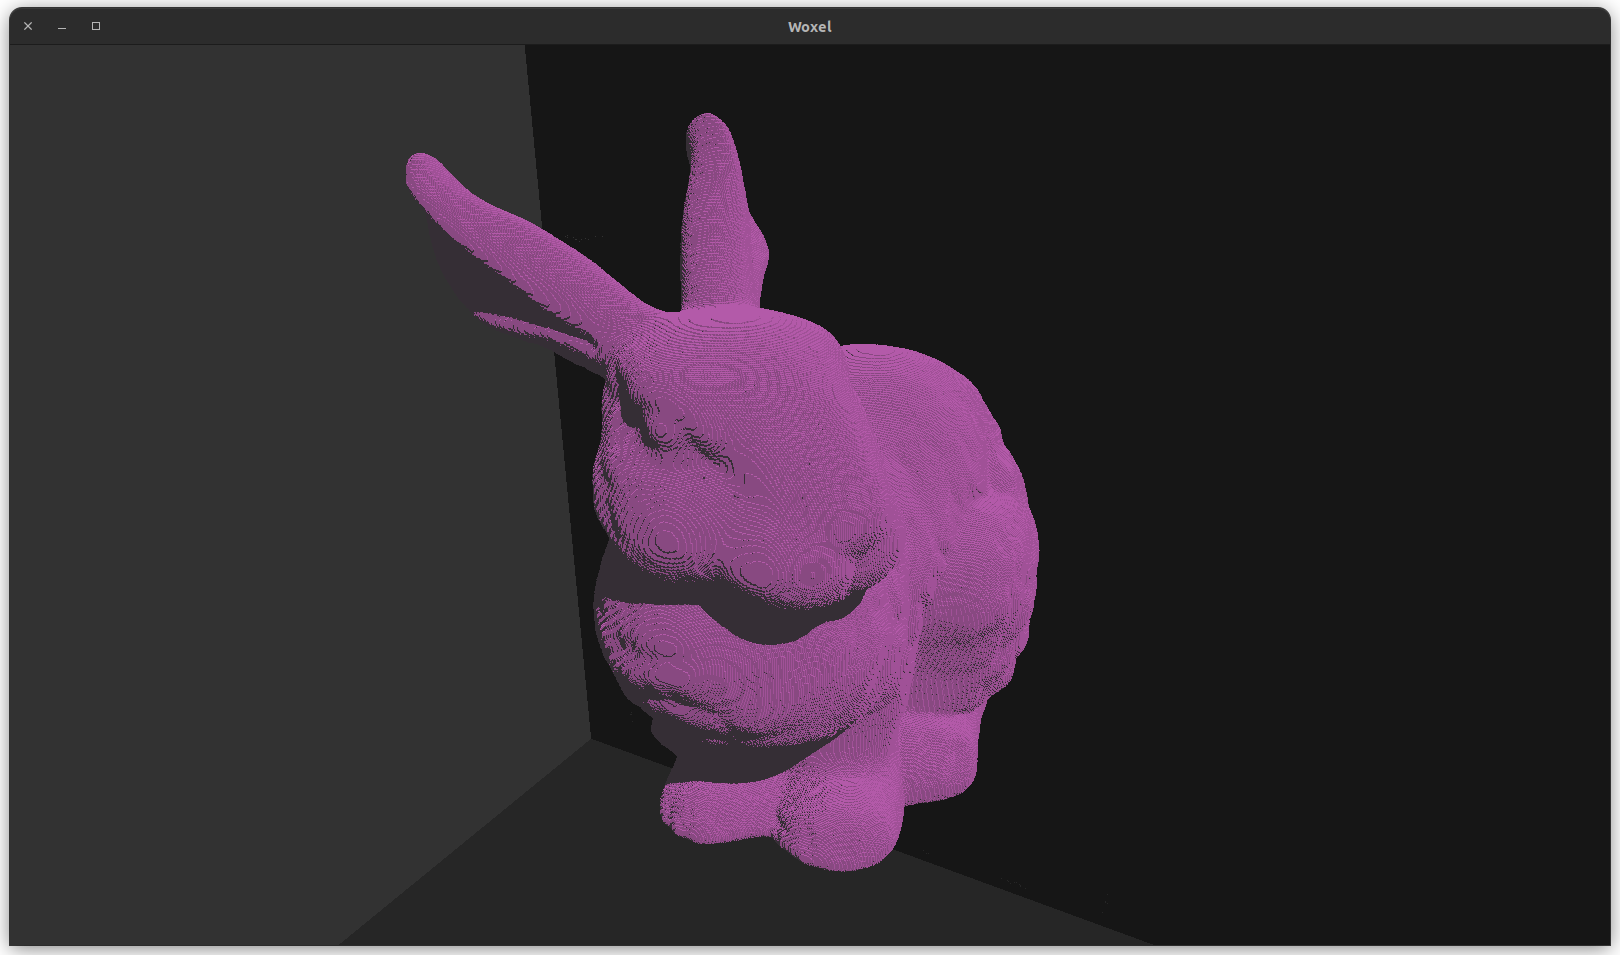
\includegraphics[width=0.8\textwidth]{bunny}
  \caption{Bunny with diffuse pink material, model voxel resolution: $628\times621\times489$}
\end{figure}

\section{Images}

This section shows some images captured in the rendering engine. All the models used are samples from the OpenVDB website\supercite{openvdb:models}. Each of the figures bellow showcase a different functionalities of the engine.

\begin{figure}[H]
  \centering
  \begin{subfigure}[b]{0.48\textwidth}
    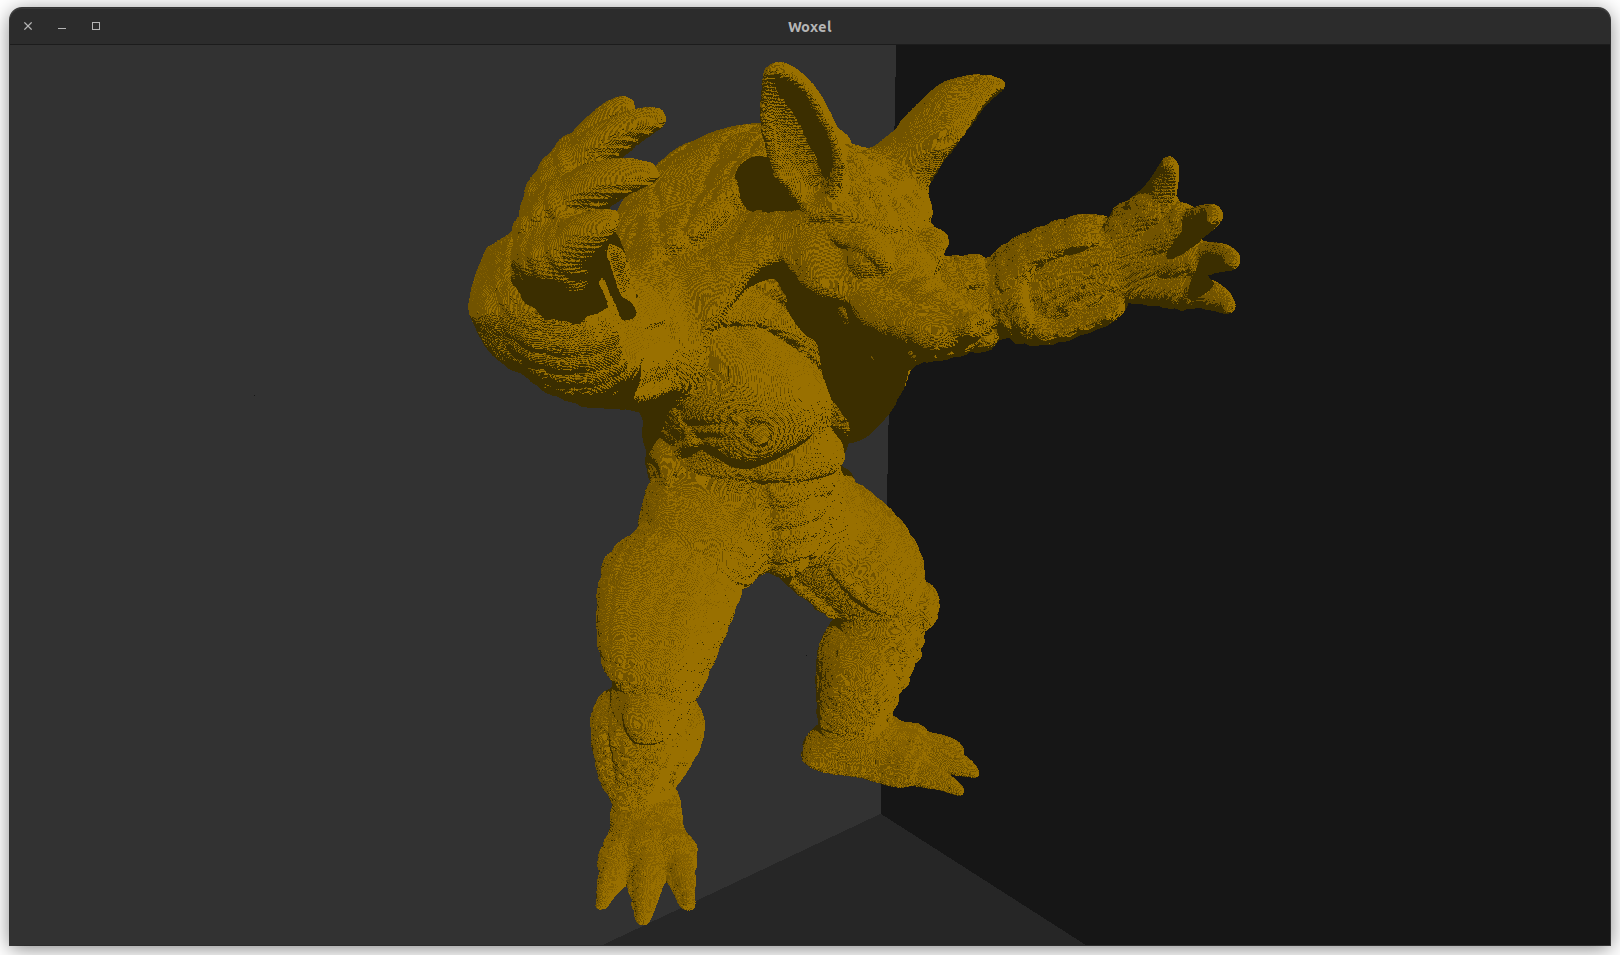
\includegraphics[width=\textwidth]{arm_1}
  \end{subfigure}
  \hfill
  \begin{subfigure}[b]{0.48\textwidth}
    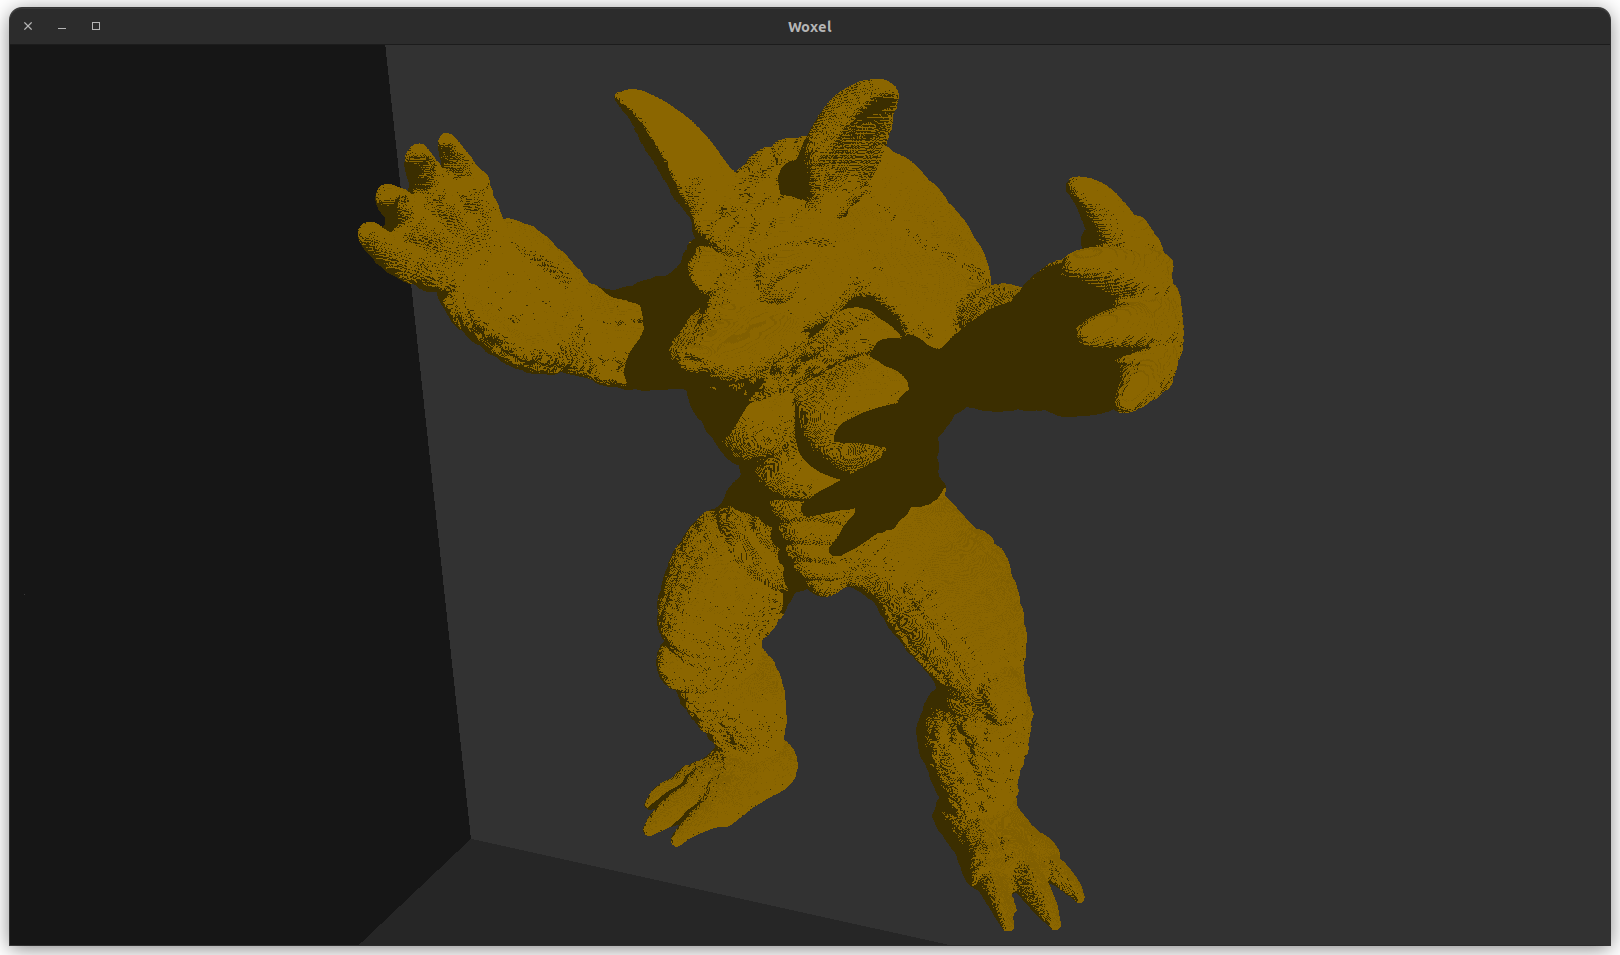
\includegraphics[width=\textwidth]{arm_2}
  \end{subfigure}
  \begin{subfigure}[b]{0.48\textwidth}
    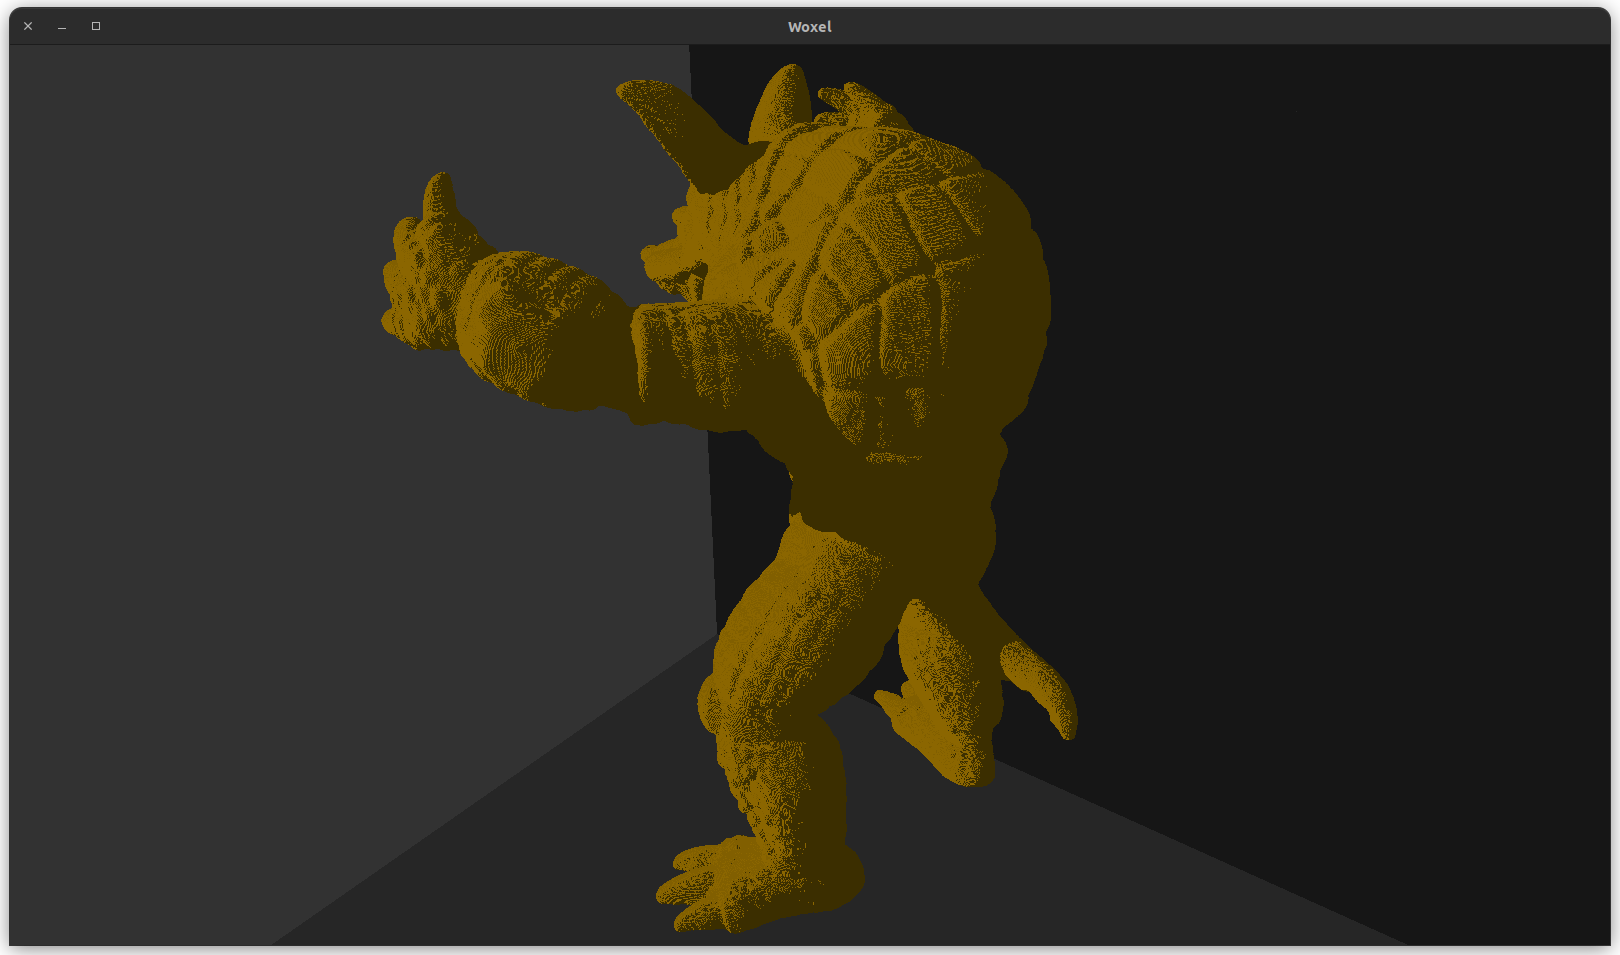
\includegraphics[width=\textwidth]{arm_3}
  \end{subfigure}
  \hfill
  \begin{subfigure}[b]{0.48\textwidth}
    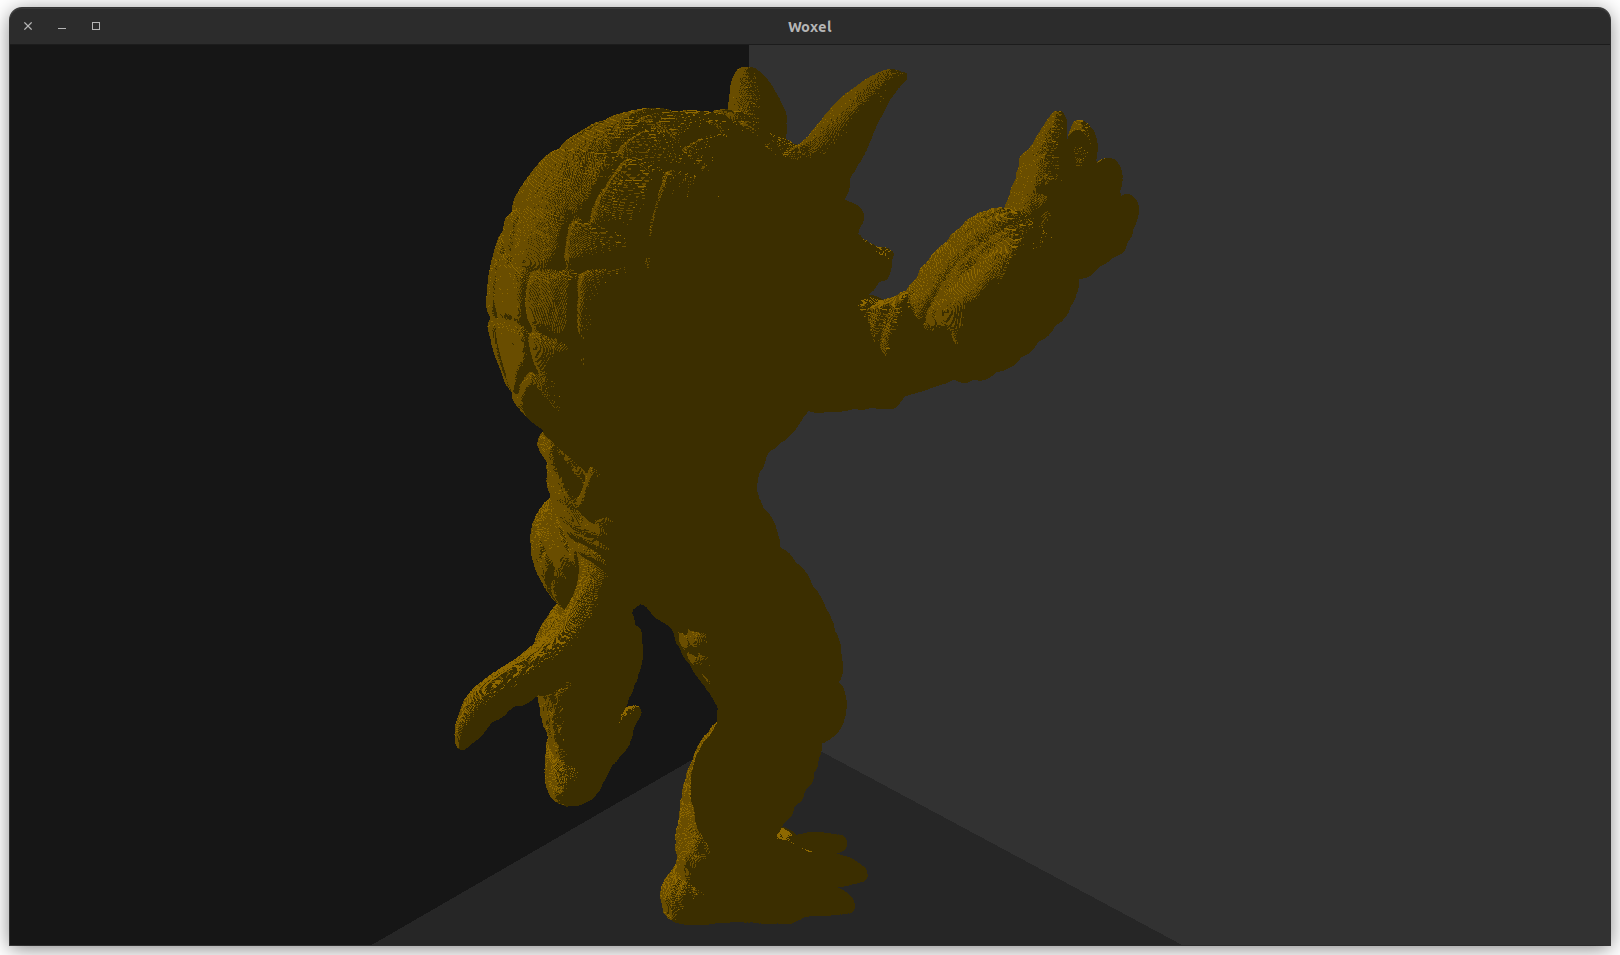
\includegraphics[width=\textwidth]{arm_4}
  \end{subfigure}
  \caption{\textbf{Multiple angles} of an armadilo model with a diffuse material. The voxel resolution of the model is $1276\times1518\times116$}
\end{figure}

\begin{figure}[H]
  \centering
  \begin{subfigure}[b]{0.48\textwidth}
    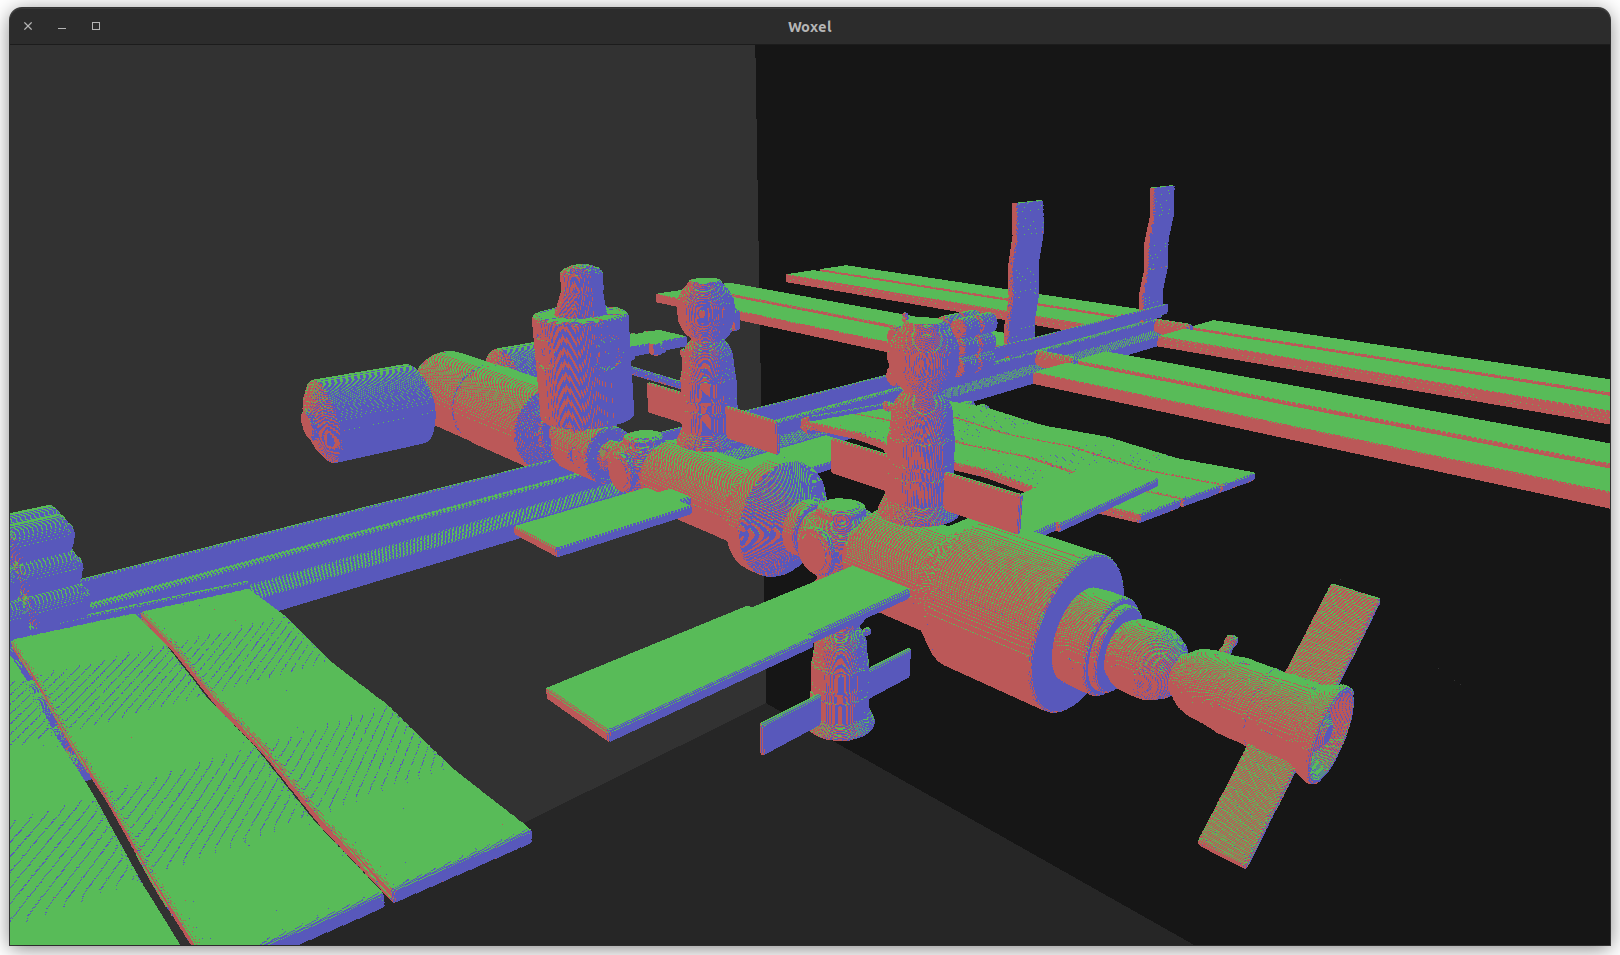
\includegraphics[width=\textwidth]{iss_rgb}
    \caption{RGB}
  \end{subfigure}
  \hfill
  \begin{subfigure}[b]{0.48\textwidth}
    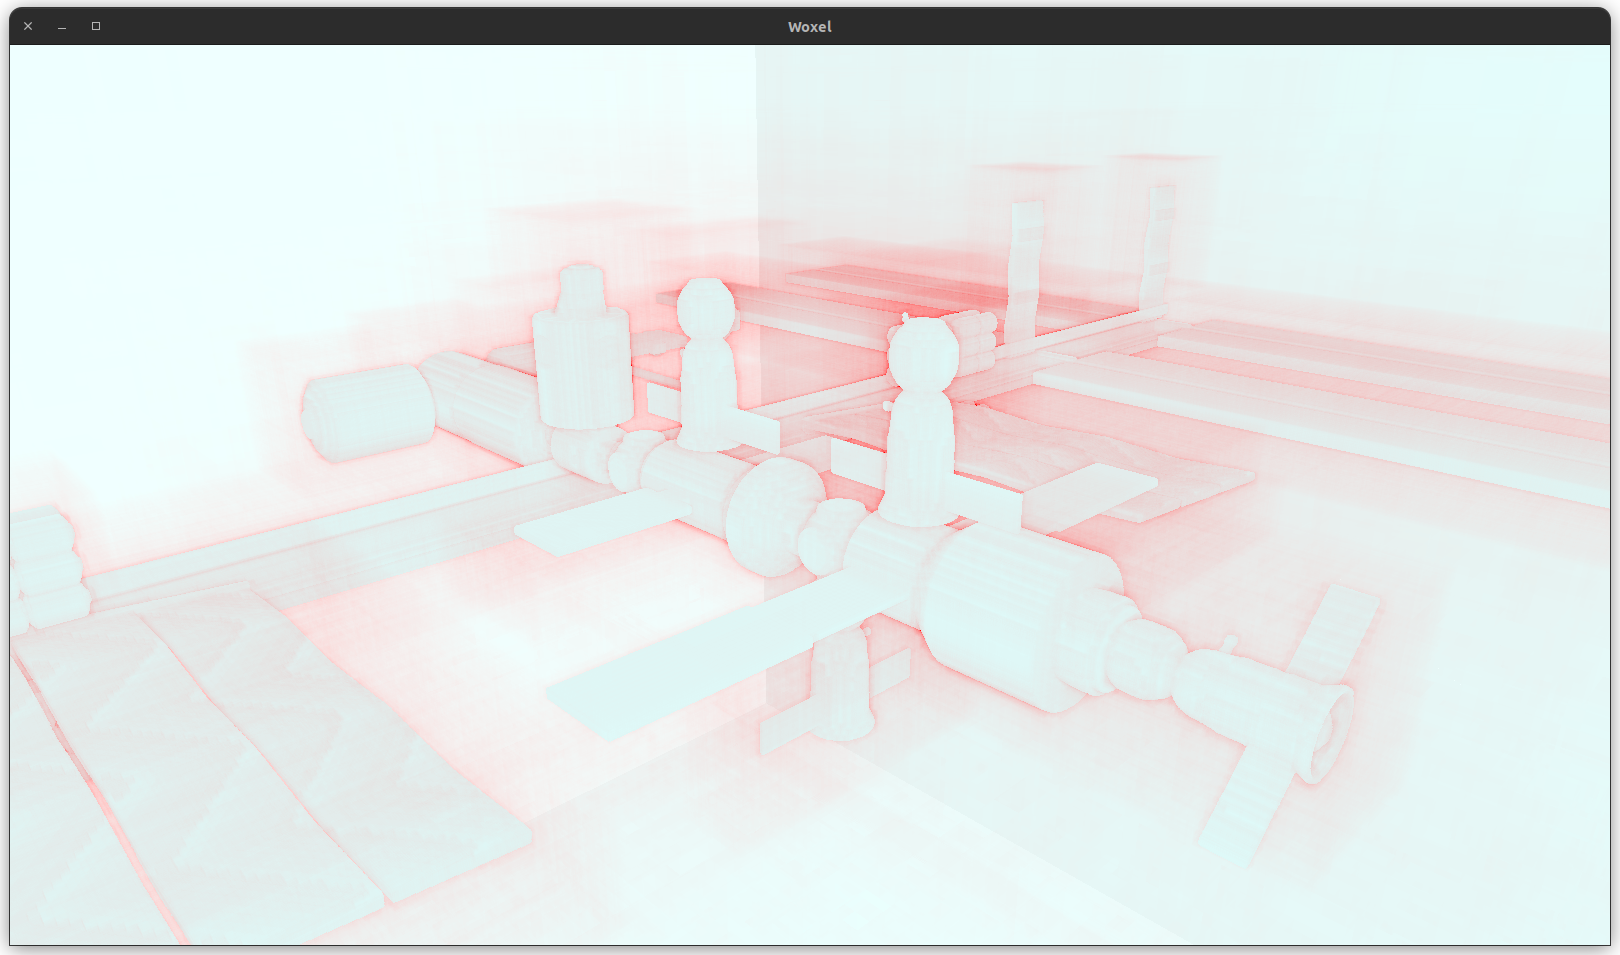
\includegraphics[width=\textwidth]{iss_ray}
    \caption{Ray}
  \end{subfigure}
  \begin{subfigure}[b]{0.48\textwidth}
    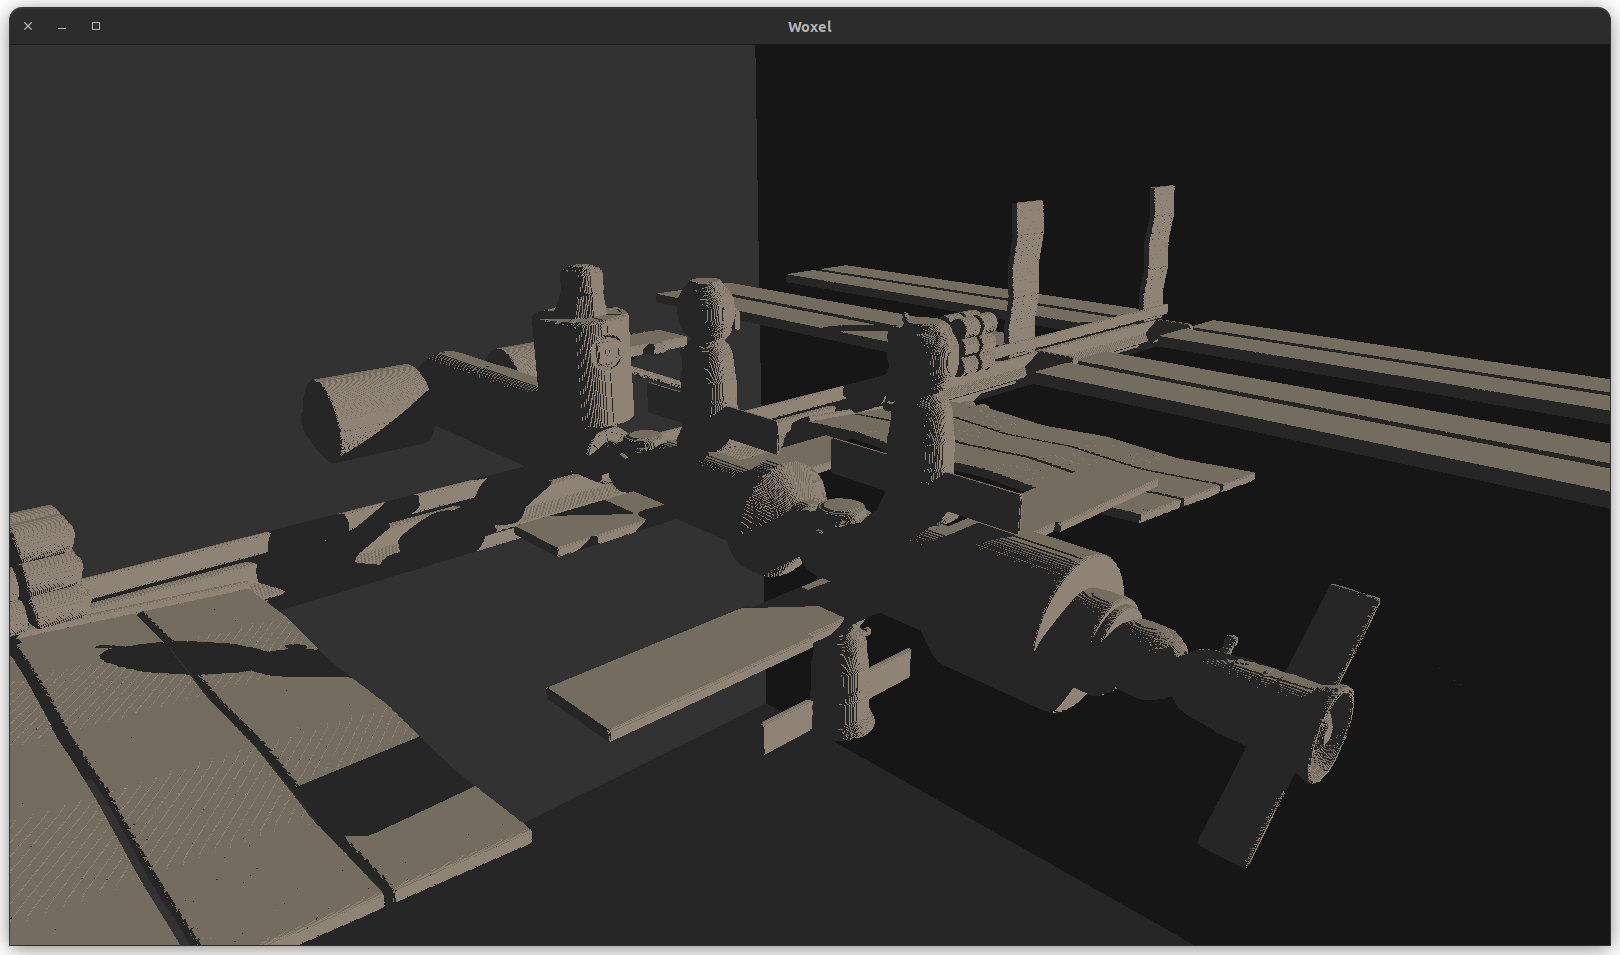
\includegraphics[width=\textwidth]{iss_diffuse}
    \caption{Diffuse}
  \end{subfigure}
  \hfill
  \begin{subfigure}[b]{0.48\textwidth}
    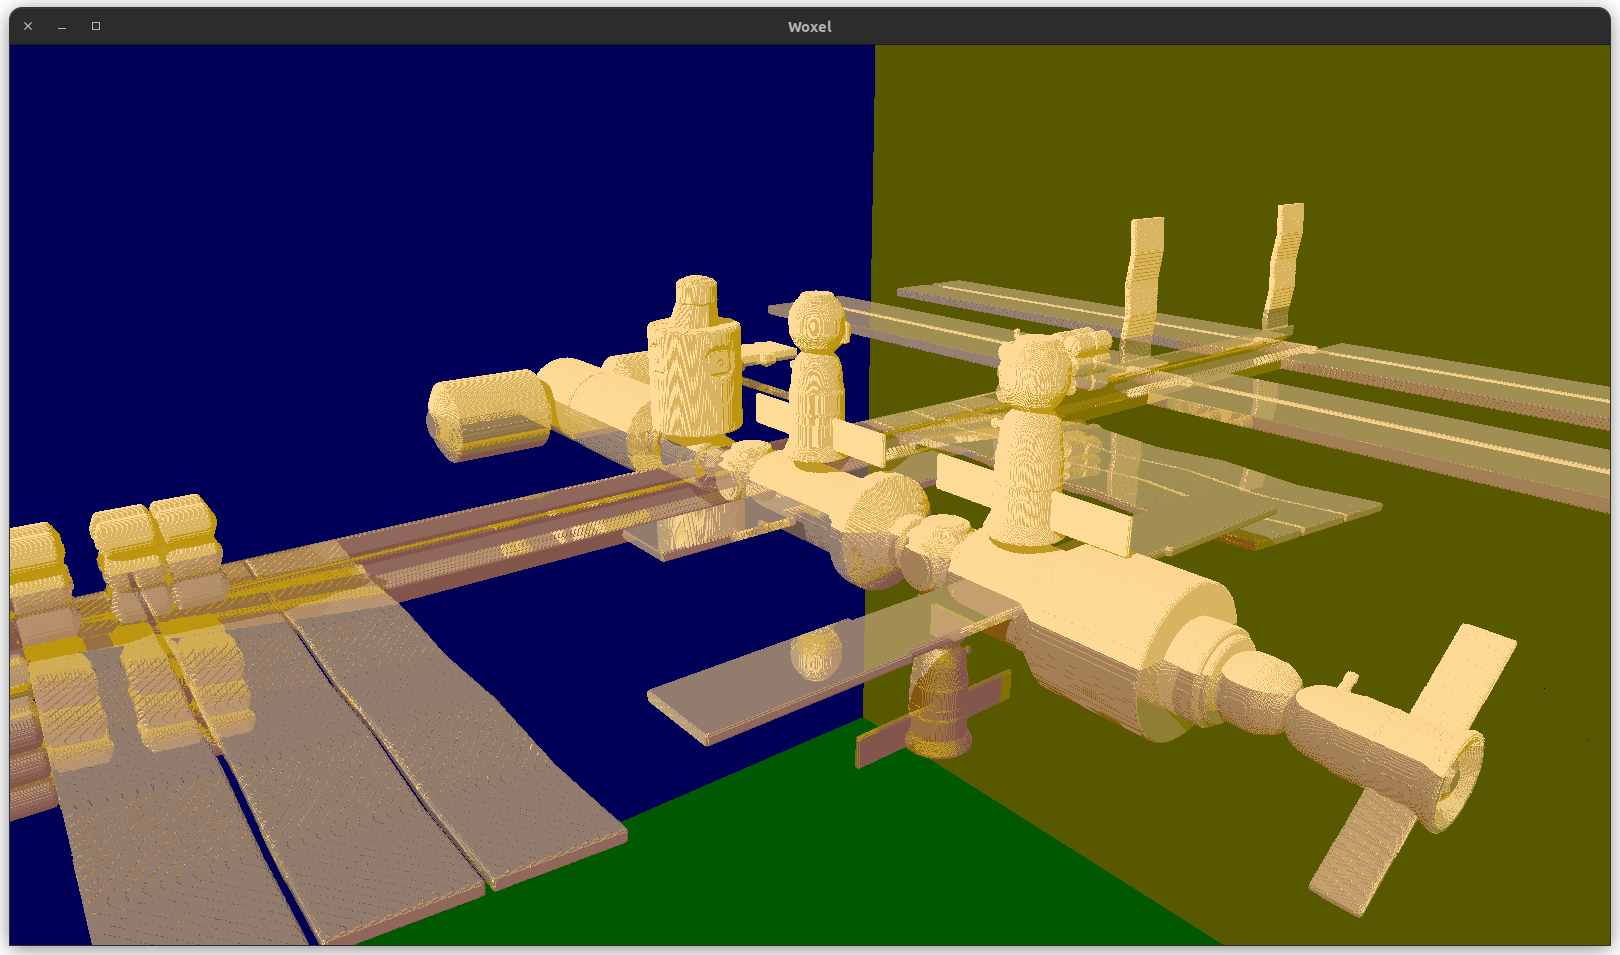
\includegraphics[width=\textwidth]{iss_gloss}
    \caption{Glossy}
  \end{subfigure}
  \caption{\textbf{Render modes} on a ISS model with voxel resolution $4561\times617\times2999$
    (a): RGB mode colors each face based on what axis it is parallel to.
    (b): Ray mode colors each pixel based on how many steps the ray took. The color is interpolated between light blue and red based on how many steps the ray took to go out of bounds or intersect a voxel. Maximum (red) is 200 steps.
    (c): Diffuse mode shows an object with diffuse material lit by sunlight.
    (d): Glossy mode shows a half glossy (bottom), half diffuse (top) model lit by sunlight. The out of bounds box is colored to discriminate which is face reflected on what surface. The reflection of the middle pod with a sphear on top can be seen in the solar panel in the middle. More reflections can be seen in the solar panels one the left and right.
  }
  \label{rendermods}
\end{figure}


\begin{figure}[H]
  \centering
  \begin{subfigure}[b]{0.48\textwidth}
    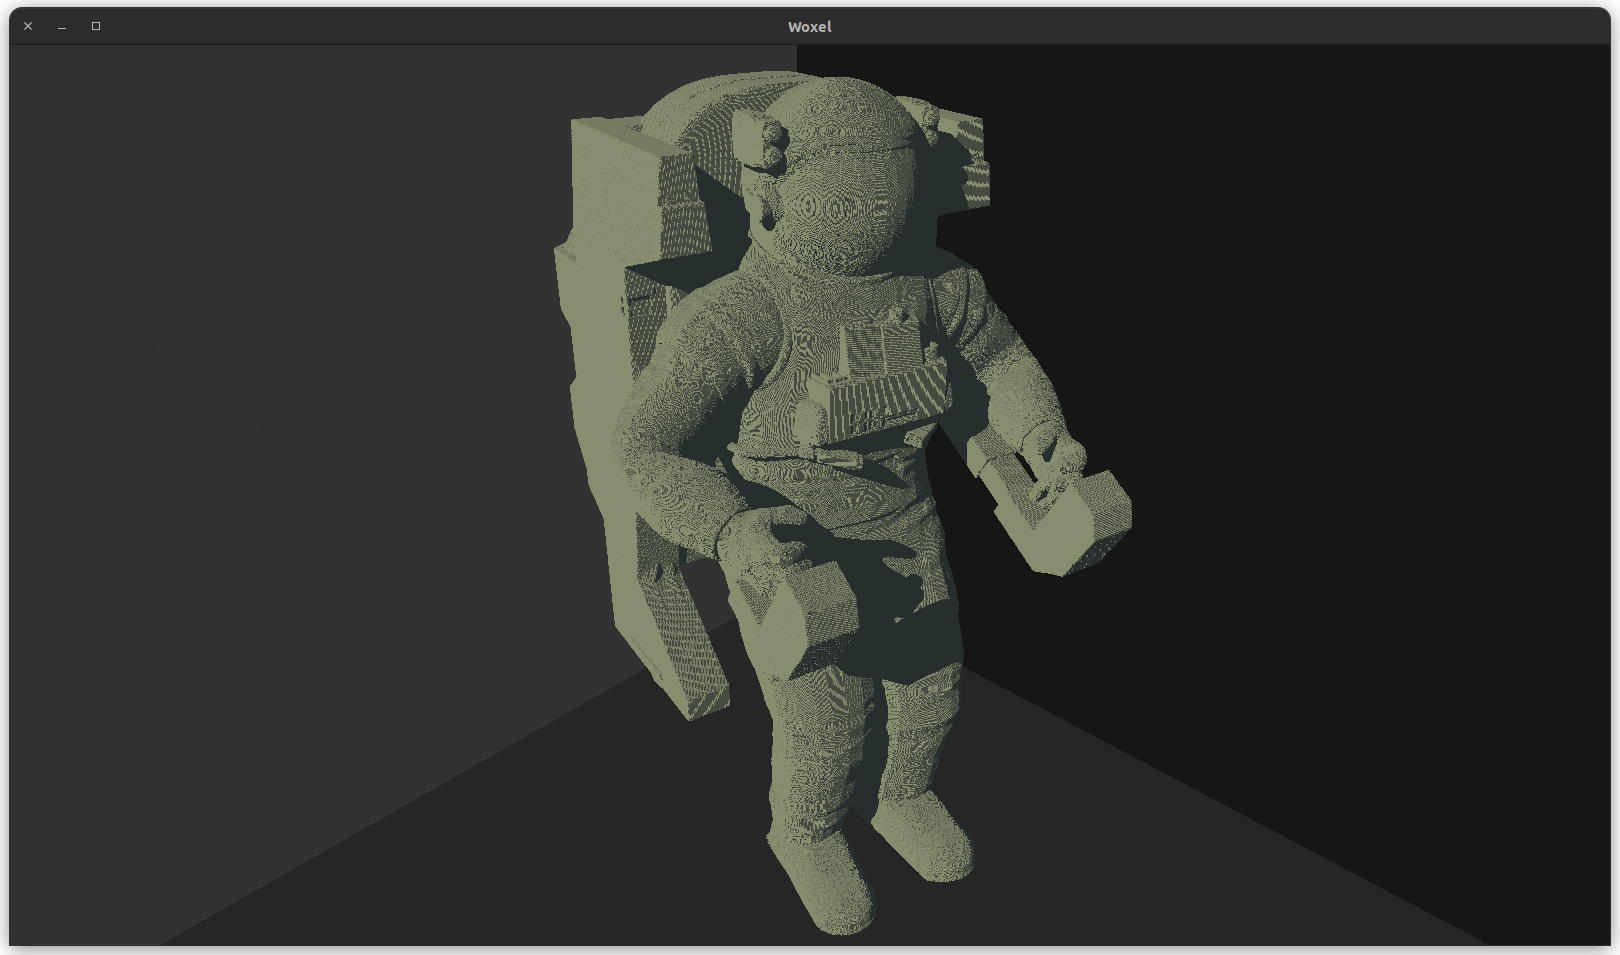
\includegraphics[width=\textwidth]{astro_1}
  \end{subfigure}
  \hfill
  \begin{subfigure}[b]{0.48\textwidth}
    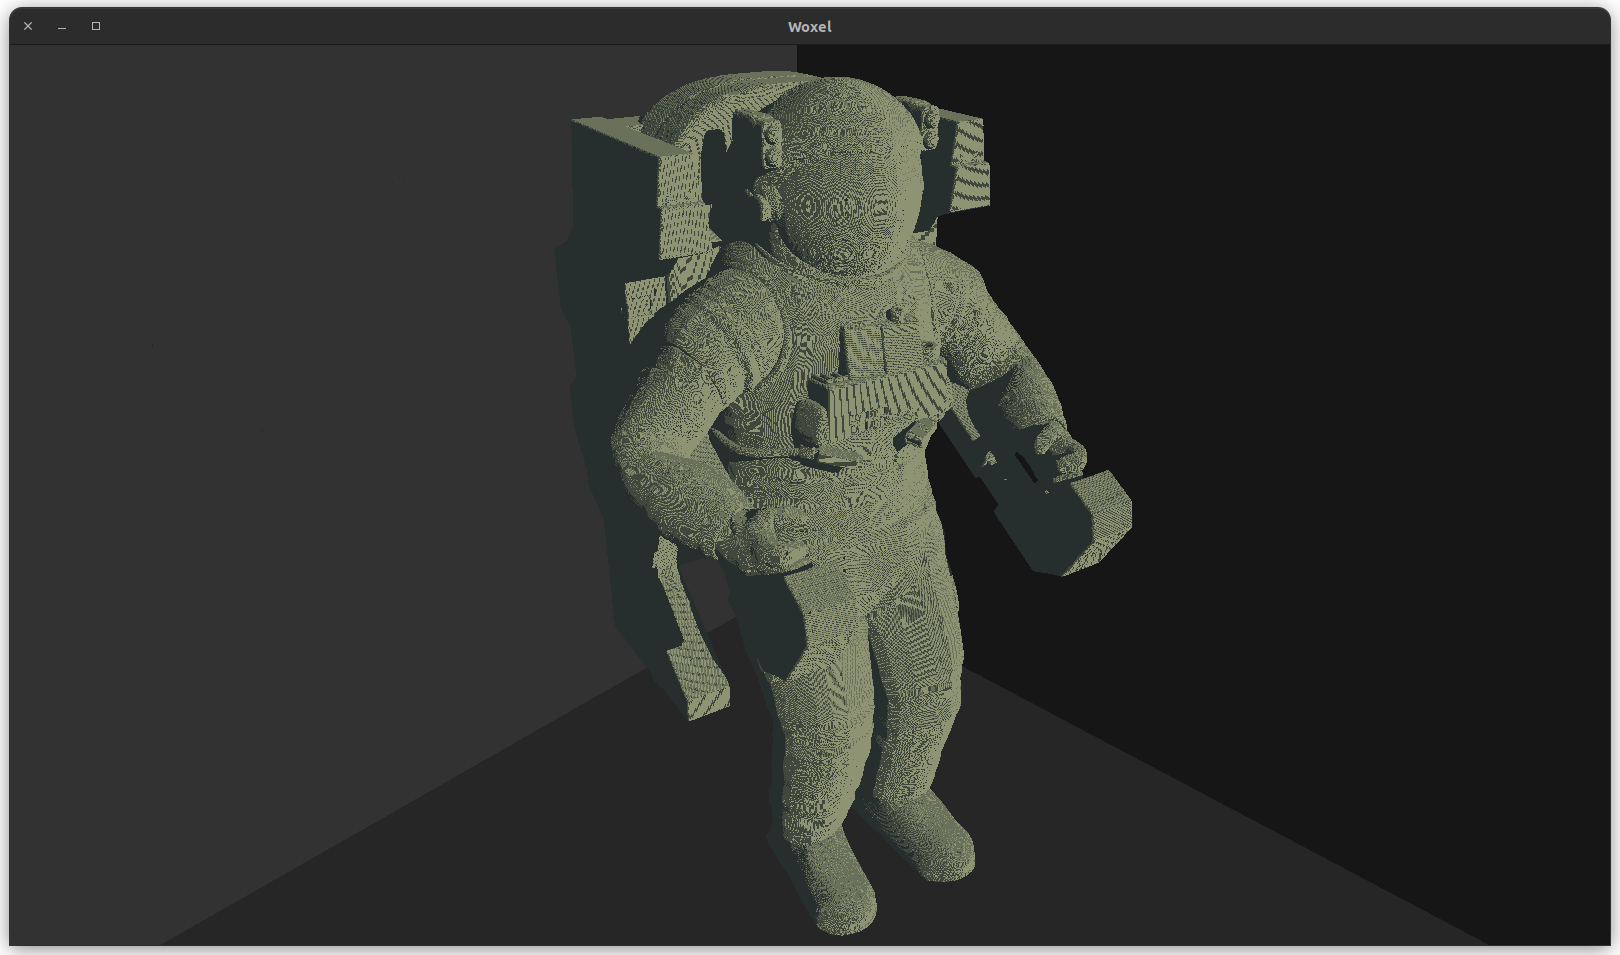
\includegraphics[width=\textwidth]{astro_2}
  \end{subfigure}
  \begin{subfigure}[b]{0.48\textwidth}
    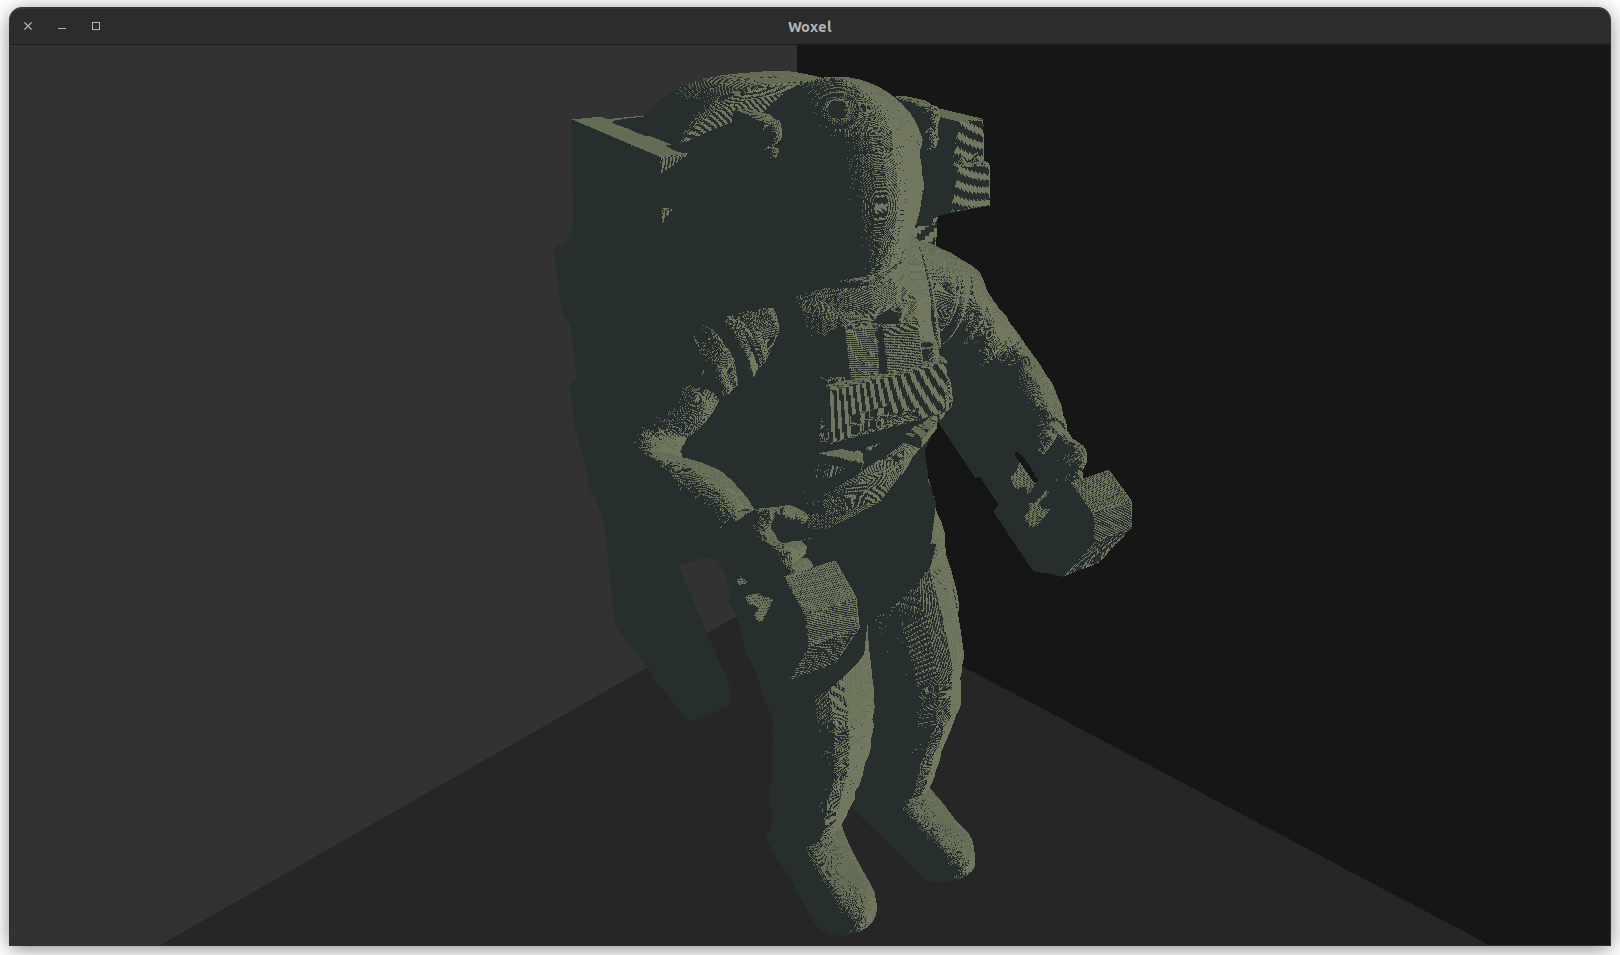
\includegraphics[width=\textwidth]{astro_3}
  \end{subfigure}
  \hfill
  \begin{subfigure}[b]{0.48\textwidth}
    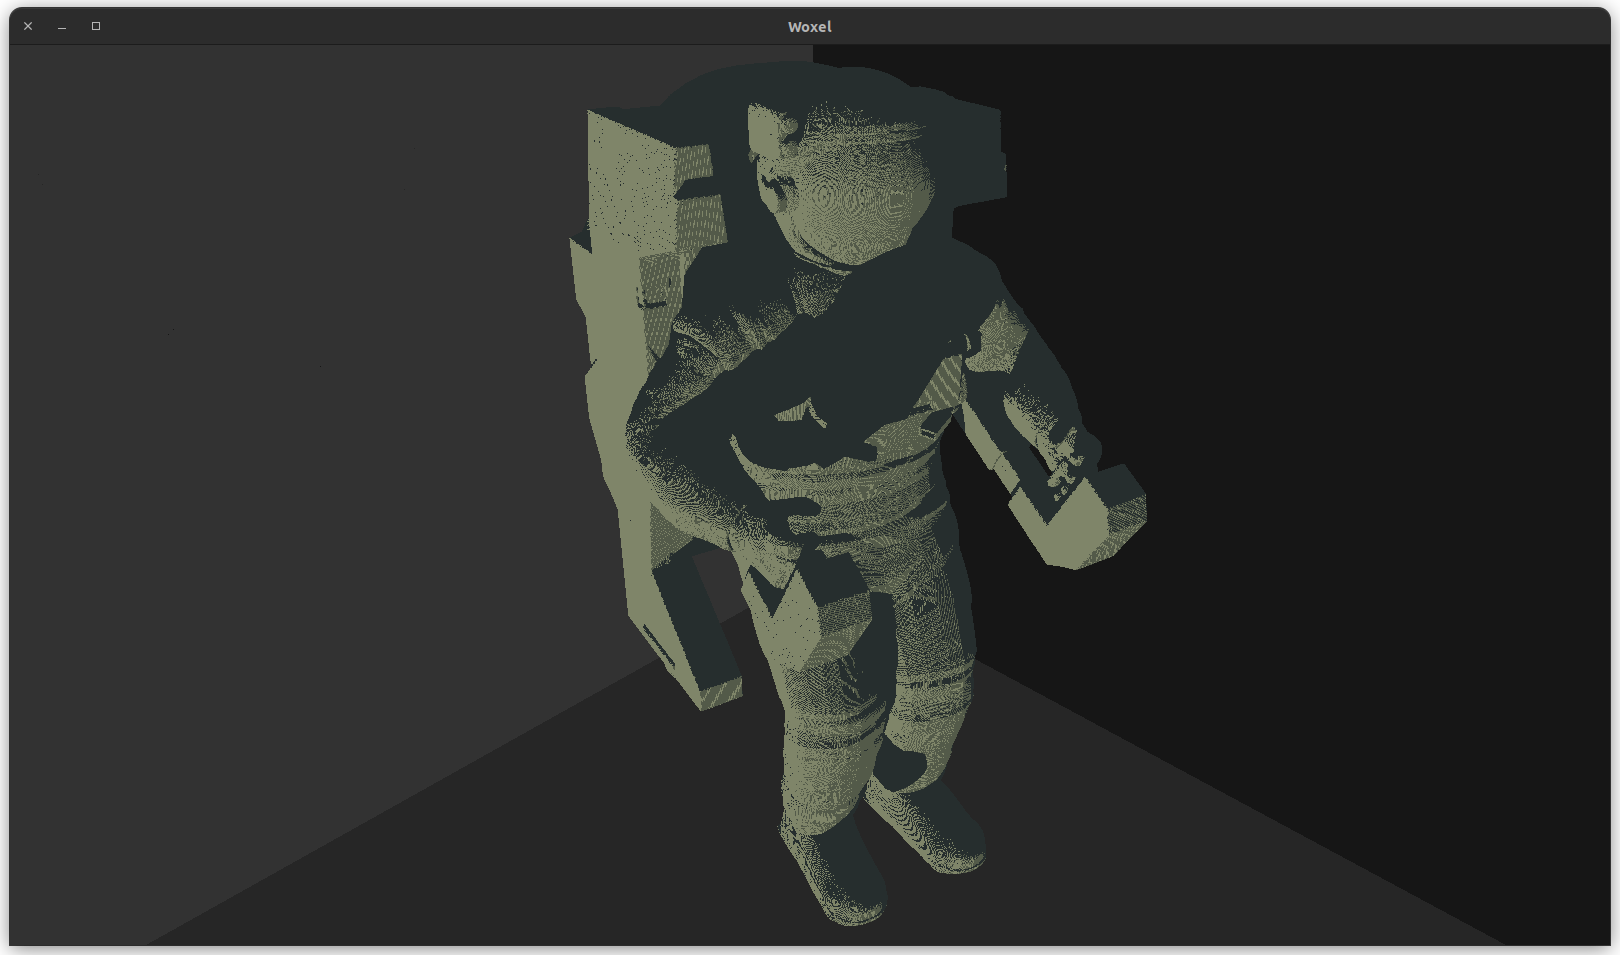
\includegraphics[width=\textwidth]{astro_4}
  \end{subfigure}
  \caption{\textbf{Dynamic Lighting} on an astronaut model. The sunlight is dynmaic, its direction, color and intensity can be changed through the developer GUI in real-time. The voxel resolution of the model is $1481\times2609\times1843$}
\end{figure}

\begin{figure}[H]
  \centering
  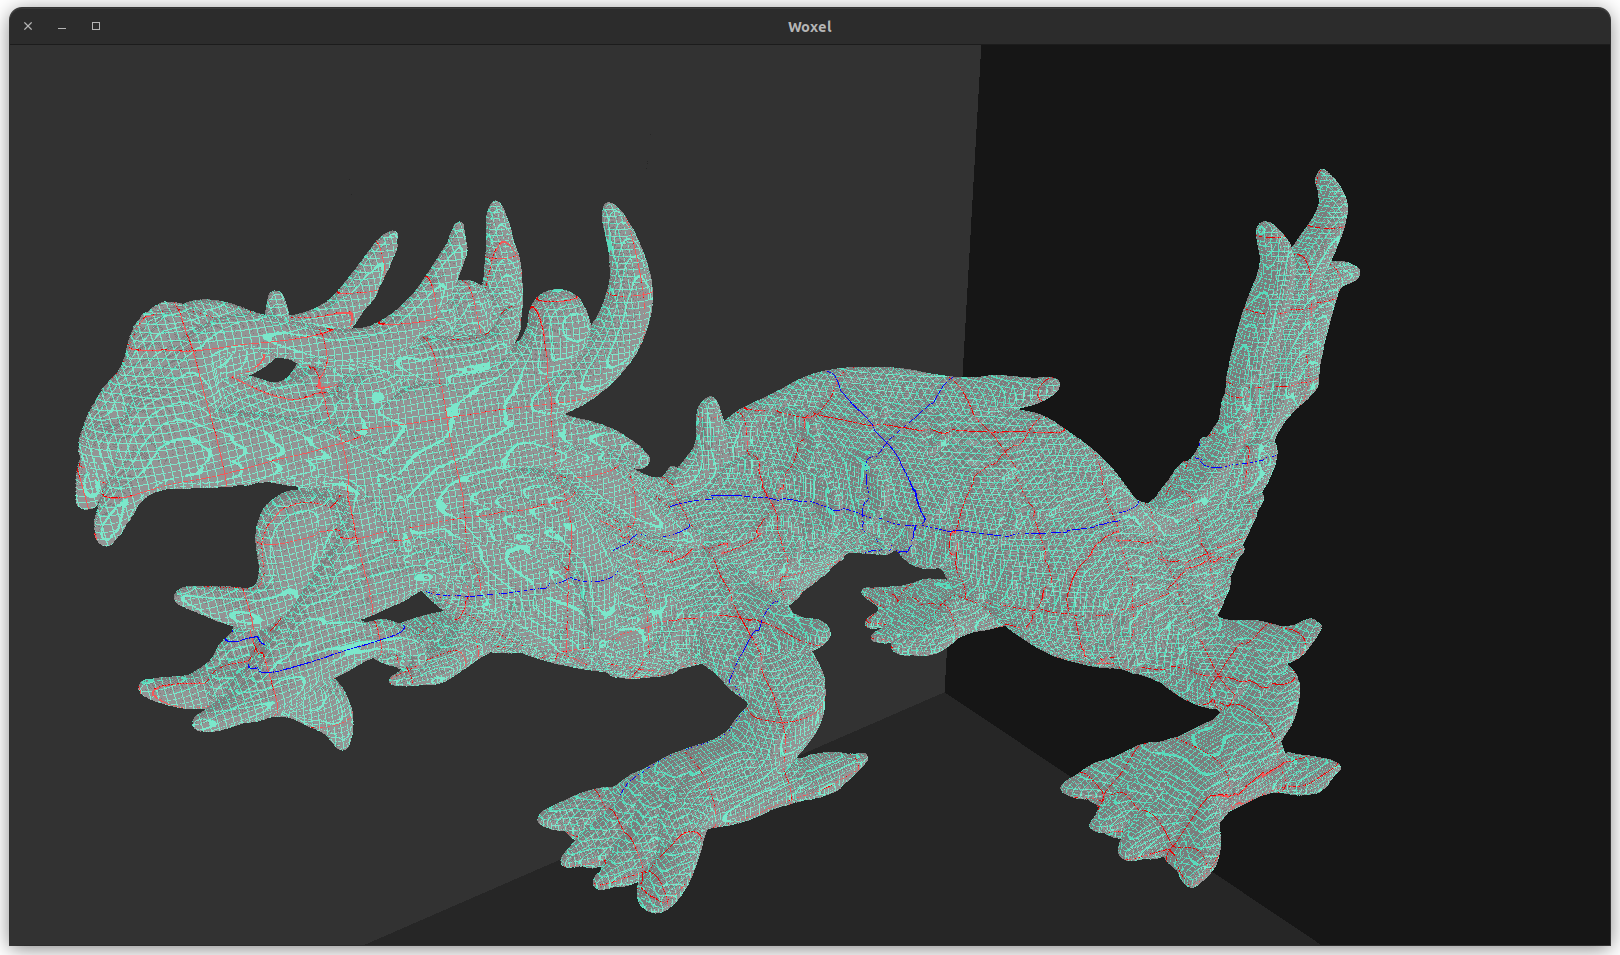
\includegraphics[width=0.8\textwidth]{dragon_3}
  \caption{\textbf{VDB highligthing}: Voxels at the boundries of VDB nodes are highlighted on a dragon model. The grid structure of the VDB can be seen at each level in the hierarchy. Node3, Node4 and Node5 boundries are shown in Cyan, Red and Blue respectively. The voxel resolution of the model is $2023\times911\times1347$}
\end{figure}

\begin{multicols}{2}[]
  \begin{figure}[H]
    \centering
    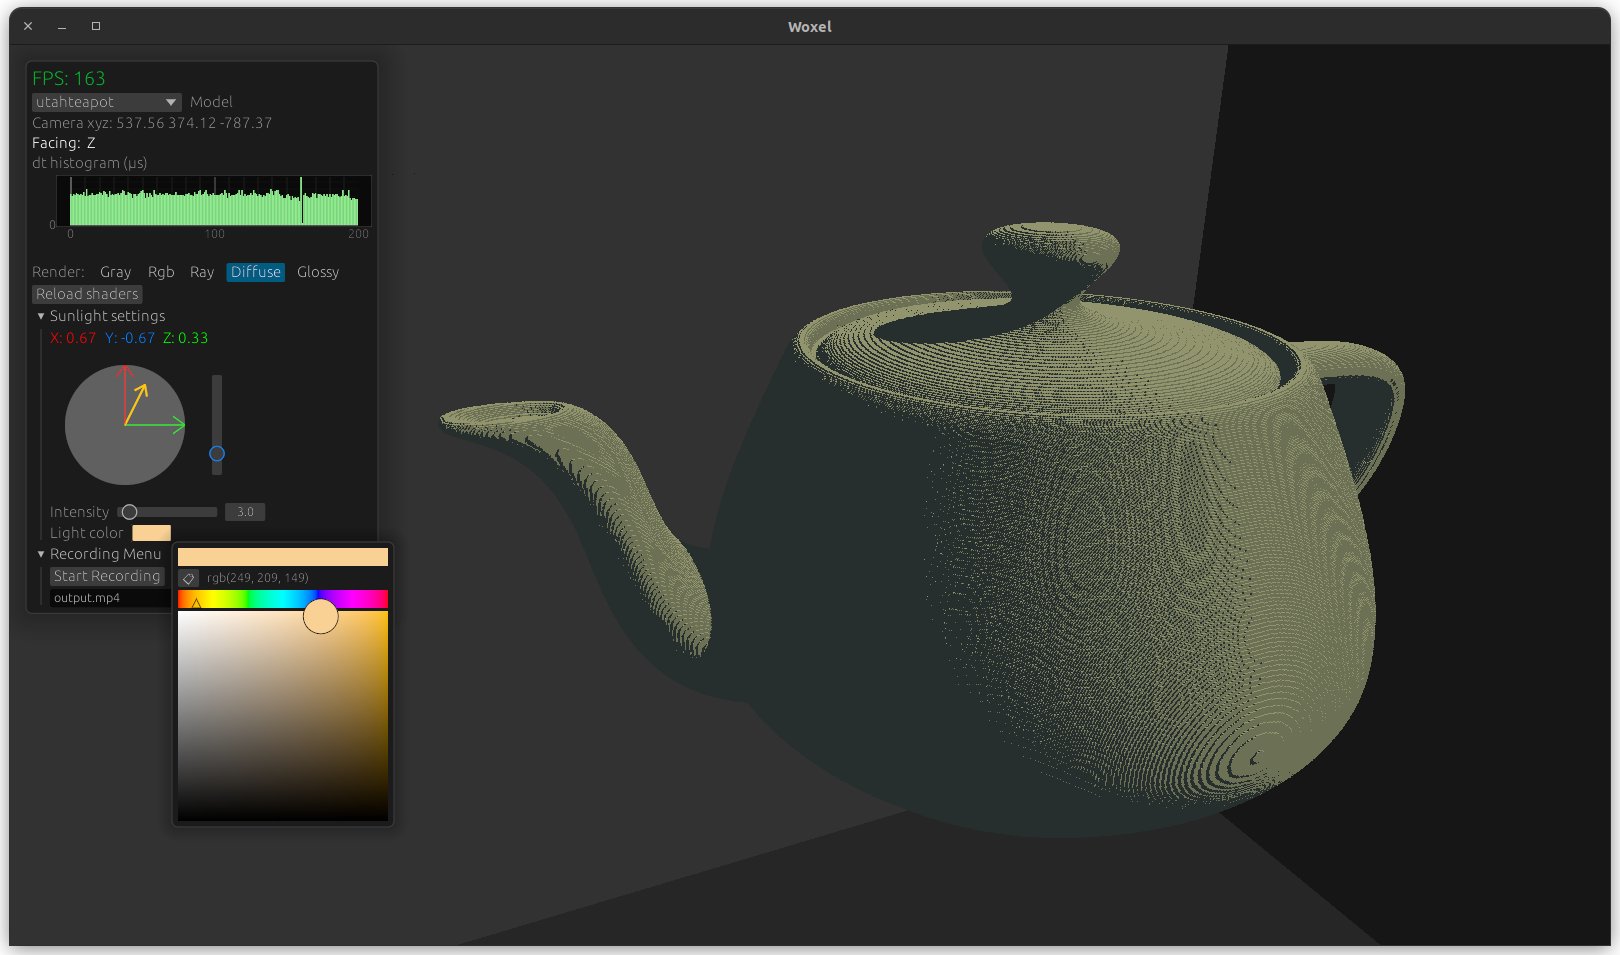
\includegraphics[width=0.96\linewidth]{gui_1}
    \caption{Developer GUI in engine}
  \end{figure}
  The developer GUI has the following uses:
  \begin{enumerate}[itemstep=0mm]
    \item Display current \acrshort{FPS} and histogram of milliseconds per frame.
    \item Changing the model in the viewport through a drop down menu that scans the assets folder for available models.
    \item Camera coordinates and facing direction
    \item Functionality to change between the render modes presented in \cref{rendermods}
    \item The option to reload the shaders while the engine is running.
    \item For the diffuse and glossy render modes there is a sunlight section available.
    \item The recording menu allows setting an output file and starting or ending the recording.
  \end{enumerate}
  \columnbreak
  \begin{figure}[H]
    \centering
    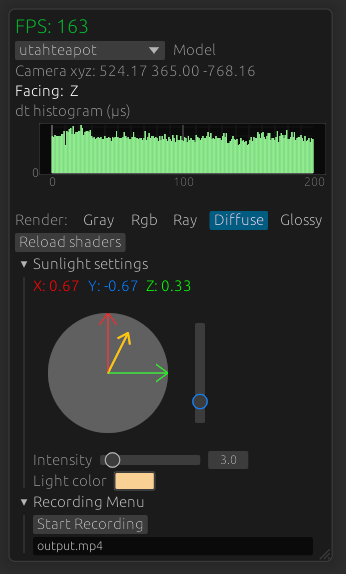
\includegraphics[width=1.0\linewidth]{gui_2}
    \caption{Developer GUI close-up}
    \label{gui}
  \end{figure}
\end{multicols}

\section{Benchmarks}
In this section the ray catsing algorithms are compared against each other on different models and render modes.

The specifications of the machine the experiments where ran on are presented in \cref{specs}.
\begin{table}[h]
  \centering
\begin{tabular}{|c||c|}
  \hline
  \multicolumn{2}{|c|}{Experiment machine specifications} \\
  \hline
  OS & Ubuntu 22.04.3 LTS x86\_64\\
  \hline
  CPU & AMD Ryzen 7 5800H with Radeon\\
  \hline
  GPU &  NVIDIA GeForce RTX 3070 Mobile\\
  \hline
  RAM & 8192MiB \\
  \hline
  FMA & Enabled \\
  \hline
\end{tabular}
  \caption{Experiment machine specifications}
  \label{specs}
\end{table}

\subsection{Comparing DDA, HDDA and HDDA+SDF}

First the average millseconds per frame are compared for the DDA, HDDA and HDDA+SDF algorithms is compared on the teapot model at 3 distinct distances from the model, one further a way, ore closer and one near the model.

\begin{table}[h]
  \centering
  \begin{tabular}{|c||c|c|c|}
    \hline
    & 2000m & 1000m & 500m \\
    \hline
    DDA & 100ms* & 100ms* & 50ms \\
    \hline
    HDDA & 9.4ms & 12.5ms & 14.4ms \\
    \hline
    HDDA & 9.4ms & 12.5ms & 14.4ms \\
    \hline
    HDDA+SDF & 6ms** & 6.4ms & 7.6ms\\
    \hline
  \end{tabular}
  \caption{Milliseconds per frame of rendering the teapot model using DDA, HDDA, HDDA+SDF at far, medium, and close distance. A voxel is considered $1\rm{m}\times1\rm{m}\time1\rm{m}$. (*): Model doesn't show in viewport because the algoirhtm exceeds the maximum step size. This time can be treated as the wors-case scenario, casting bouncing the maximum number of times for each pixel. (**): Frame rate cap is hit at 165 FPS}
\end{table}

\section{Future work}
\section{Final remarks}

\include{chapters/conclusion.tex}

%%%%%%%%%%%%%%%%%% REFERRENCES %%%%%%%%%%%%%%%%%%
\printbibliography[title={References},heading=bibintoc]


%%%%%%%%%%%%%%%%%% ACRONYMS %%%%%%%%%%%%%%%%%%
\newpage
\printglossary[type=\acronymtype]

%%%%%%%%%%%%%%%%%% APPENDICES %%%%%%%%%%%%%%%%%%
\begin{uomappendix}
    \section{Project outline}
    Project outline as submitted at the start of the project is a required appendix.

    \section{Risk assessment}
    Risk assessment is a required appendix. Put here. And there as well
\end{uomappendix}

\end{document}
